\documentclass[a4paper,twoside,11pt]{report}
%\documentclass[a4paper,oneside,11pt]{report}
\def\lingua{english}
\usepackage[T1]{fontenc}
\usepackage{graphicx}
\usepackage{epsfig}
\usepackage{ia_urb_thesis}
\usepackage[\lingua]{babel}
\usepackage{longtable}
\usepackage{booktabs}

\begin{document}

\titolo{Containerizing The Cloud For\\[5mm]
        Managing Applications At Scale}
\candidato{Antonio Esposito}
\relatore{Chiar.mo Prof.~Alessandro Bogliolo}
\correlatori{Dott.~Luca Ferroni \\
             Dott.~Andrea Seraghiti \\
             Dott.~Saverio Delpriori}
\annoaccademico{2014-2015}

\copertinatesi
\dedica{To my parents}
\indice
\indicefigure
\indicetabelle
\iniziatesto

This work is licensed under a \textit{Creative Commons Attribution-ShareAlike 4.0 International License} https://creativecommons.org/licenses/by-sa/4.0/legalcode

\chapter{Introduction}\label{introduction}

Today there is the \emph{cloud}, where some kind of services are
delegated by third-party providers. There are structured mainly 3
different kind of services, depends on abstraction level:

\begin{itemize}
\itemsep1pt\parskip0pt\parsep0pt
\item
  \emph{Infrastructure as a Service} (IaaS) for raw compute, network,
  storage and other low-level needs
\item
  \emph{Platform as a Service} (PaaS) for running applications by
  software developers
\item
  \emph{Software as a Service} (SaaS) for provide applications to end
  users
\end{itemize}

Anyway, even if cloud resoles a necessity sometimes there is the need of
avoid \emph{outsourcing}, or using directly cloud technologies for
providing services to customers.

\section{Goal}\label{goal}

Luckily, today there is a vast availability of free software for
reproduce some cloud services.

Starting from an overview of software development, systems management,
software architectures and application environments, it will be provided
some guidelines and researched existing available solutions, with the
goal of following the process of PaaS management built on top of an
IaaS, in a modern and scalable way, guaranteeing the governance through
monitoring.

The final goal is providing SaaS through a suitable environment for
running applications. For this purpose, it will be used an application
as case of study: \emph{Gasista Felice}.

This solution will integrate:

\begin{itemize}
\itemsep1pt\parskip0pt\parsep0pt
\item
  configuration of a IaaS
\item
  describing in a declarative way the PaaS resources
\item
  monitoring and benchmarking the live management of the whole platform
  when the application will be in execution
\end{itemize}

The examined and studied solution covers the current state of art, in
particular consists of \emph{Kubernetes} developed from Google's
Engineers, RedHat's \emph{OpenShift}, but also \emph{CoreOS} from the
namesake company, and HashiCorp's \emph{Terraform}.

All the project comes as free software and are released on the GitHub
portal.

\section{Organization}\label{organization}

Chapter 2 introduces the working environment in which this thesis was
born and the technological context for which was conceived.

Chapter 3 introduces containers' core concepts and the application to
the use case.

Chapter 4 describes how to bootstrap a IaaS/PaaS providing a production
environment.

Chapter 5 describes the stack of PaaS showing how applications could
take advantage on it.

Chapter 6 shows how to control, monitor, analyze, and visualize data
about applications.

Chapter 7 does a summary of this experience, and present some potential
evolution of this project in order to achieve further targets.
\chapter{Background}\label{background}

This chapter introduces the technological context in which this thesis
was born with some references to the working environment in which it is
implemented.

Since this document covers the workflow from designing application
architecture in containers to deploying it in a real production
environment, as well as using the application in development and QA
environments, the context is presented from multiple points of view:

\begin{itemize}
\itemsep1pt\parskip0pt\parsep0pt
\item
  the automation of the IT operations
\item
  the evolution of the development workflow
\item
  the scalability of architectures in the cloud
\item
  the flexibility of multiple environments
\item
  the key factors of Free Software and Sharing Economy that has led
  useful tools and practices used to develop the project
\end{itemize}

\section{Manageability in IT
Operations}\label{manageability-in-it-operations}

The definition of IaaS from Wikipedia\cite{CloudComputing}:

\begin{quote}
In the most basic cloud-service model {[}\ldots{}{]} providers of IaaS
offer computers -- physical or (more often) virtual machines -- and
other resources. {[}\ldots{}{]}
\end{quote}

Common GNU/Linux distributions comes with a built-in package manager
that provides a powerful entrypoint for installing and managing
packages, from libraries to graphical applications. Using this feature,
historically system administrators managed servers (IaaS)
\emph{manually} directly via shell, upgrading the system, installing and
configuring the necessary packages. This approach introduces human
errors and non reproducible operations, so it's flacking when scaling
the numbers of engineers, hosts, applications and tasks. For example,
it's difficult evolving the environment changing all configurations,
because there is not a formal way to do it.

Even if the manual management is immediate and doesn't need
(pre)organizations, it has several limits. A first step derives from
other industrial revolutions, minimizing the human intervation and
\emph{automating} all operations as possible, via \emph{scripting} or
dedicated tools for \emph{application deployment} and
\emph{configuration management} (e.g.: Chef, Puppet, SaltStack,
Ansible). So humans doesn't do things directly, but instruct machines to
do it in a more efficient, reproducible and reliable way. A consequence
of this, there is the \emph{Pets vs Cattle} contrast, seeing the
opposition of who thinks the server hostnames should be choice
creatively (as pets) or in a more industrial and pragmatic way (as
cattle).

Even if this approach worked for years at scale, the application level
remains coupled to underlying infrastructure. In \emph{PaaS}, instead,
there is a strong separation of infrastructure and application levels.

From Wikipedia:

\begin{quote}
In the PaaS models, cloud providers deliver a computing platform,
typically including operating system, programming-language execution
environment, database, and web server. Application developers can
develop and run their software solutions on a cloud platform without the
cost and complexity of buying and managing the underlying hardware and
software layers. {[}\ldots{}{]}
\end{quote}

In 2009 \emph{Ian Murdock}, the Debian founder, in its article \emph{Do
operating systems still matter?}\cite{DoOperatingSystemsStillMatter}
concluded that today developers using a PaaS are not more concerned
about underlying hardware or operating system related features, but also
about platform-level exposed features, so operating systems should be
rethinked in order to expose a better, more integrated higher level
experience.

Also RedHat in \emph{The Platform Abstraction Advantage of
PaaS}\cite{ThePlatformAbstractionAdvantageOfPaaS} concludes with the
following:

\begin{quote}
Clearly, platform abstraction solves more problems for IT than an IaaS+
approach. Enterprises embrace cloud for agility benefits and having an
abstraction at the platform layer maximizes these benefits. DevOps is
more attractive for enterprises because their IT can now deliver at the
speed of business and the standardization of application development
platform through abstraction at higher layers of stack and self service
option for developers enables IT to meet the business needs.
\end{quote}

\begin{longtable}[c]{@{}lll@{}}
\caption{Summary of Evolution in IT Operations}\tabularnewline
\toprule
Model & Operations & IaaS/SaaS strong separation\tabularnewline
\midrule
\endfirsthead
\toprule
Model & Operations & IaaS/SaaS strong separation\tabularnewline
\midrule
\endhead
IaaS & manual & no\tabularnewline
IaaS+ & automation & no\tabularnewline
PaaS & automation & yes\tabularnewline
\bottomrule
\end{longtable}

\begin{figure}[htbp]
\centering
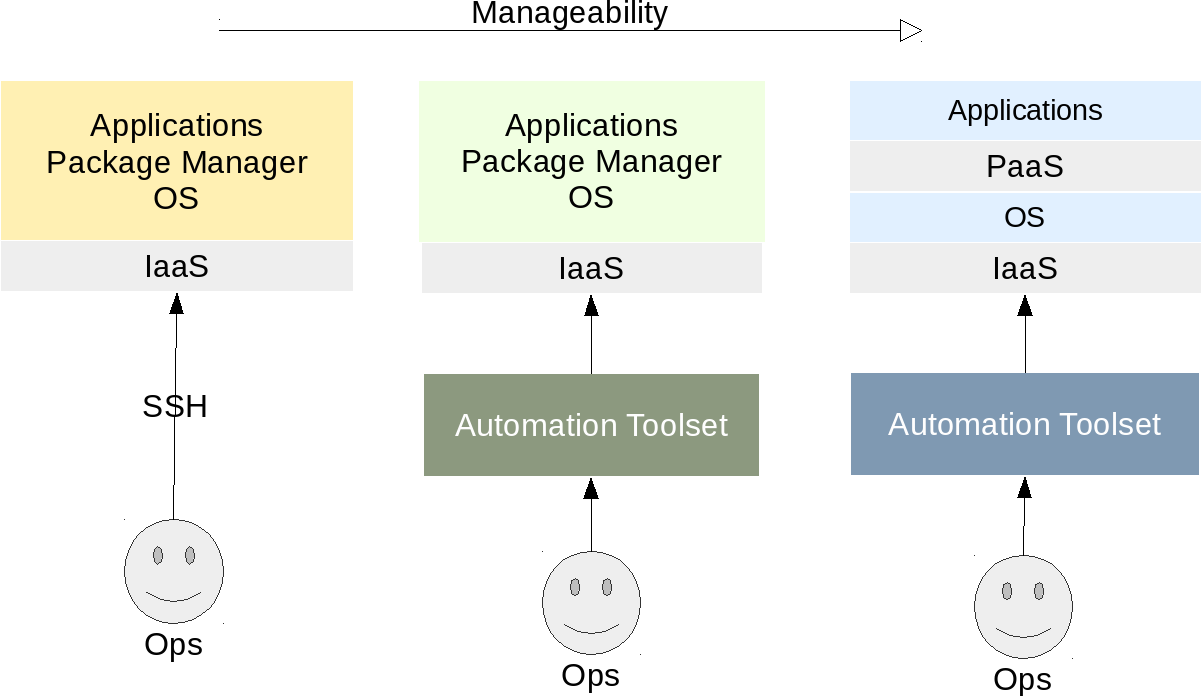
\includegraphics{media/ch2-paas.png}
\caption{Evolution in IT Operations}
\end{figure}

\section{Velocity in Development
Workflow}\label{velocity-in-development-workflow}

In 2001 was published the \emph{Agile Manifesto}, a set of 12 principles
that represent a first step towards a faster and more efficient approach
to developers needs, going beyond the traditional \emph{waterfall}
development. From development workflow, it's based on a \emph{Continuous
Integration} (CI) system running tests automatically, notifying to users
when fails.

While Agile methodologies made the development faster, the users will
not receive this since delivery of applications remains slow. That
create the necessity for a more collaboration/interaction between
development and operations/delivery teams in order to automating the
application deployment as soon as it passed the tests. This is called
\emph{Continuous Delivery}, extending the CI concept to production.

Consequently, also development and production environment should getting
close, aim to the so called \emph{dev/prod parity}. This way to build
applications was formerly by Heroku, popular PaaS, with \emph{The
Twelve-Factor App} (http://12factor.net/), a 12 good practices to apply
at SaaS. Separate cleary development and operations through a contract,
and represent the beginning of DevOps era. Other PaaS shared and was
born on top of these principles, such as \emph{Deis} or
\emph{OpenShift}.

In a DevOps context there are usually at least these components:

\begin{itemize}
\itemsep1pt\parskip0pt\parsep0pt
\item
  \emph{Source Code Management} provides repositories hosting for Git
  (or other source code versioning system) projects (e.g.: \emph{Gogs},
  \emph{GitLab})
\item
  \emph{Continuous Integration/Continuous Delivery} execute automated
  tests and send somewhere else when software is ready to deploy in
  staging, QA or production environment (e.g.: \emph{Travis CI},
  \emph{GitLab CI}, \emph{Drone}, \emph{Jenkins})
\item
  \emph{Platform as a Service} is the core of infrastructure and
  automatically manage the applications, including the upgrade, some
  monitoring features (e.g.: \emph{Deis}, \emph{OpenShift})
\end{itemize}

References:

\begin{itemize}
\itemsep1pt\parskip0pt\parsep0pt
\item
  http://radar.oreilly.com/2012/06/what-is-devops.html
\item
  http://somic.org/2010/10/06/devops-and-sysadmin/
\item
  http://theagileadmin.com/what-is-devops/
\end{itemize}

\begin{longtable}[c]{@{}lll@{}}
\caption{Summary of Evolution in Development Workflow}\tabularnewline
\toprule
Workflow & Development cycles & Delivery cycles\tabularnewline
\midrule
\endfirsthead
\toprule
Workflow & Development cycles & Delivery cycles\tabularnewline
\midrule
\endhead
Waterfall & long & long\tabularnewline
Agile & short (CI) & long\tabularnewline
DevOps & short (CI) & short (CD)\tabularnewline
\bottomrule
\end{longtable}

\begin{figure}[htbp]
\centering
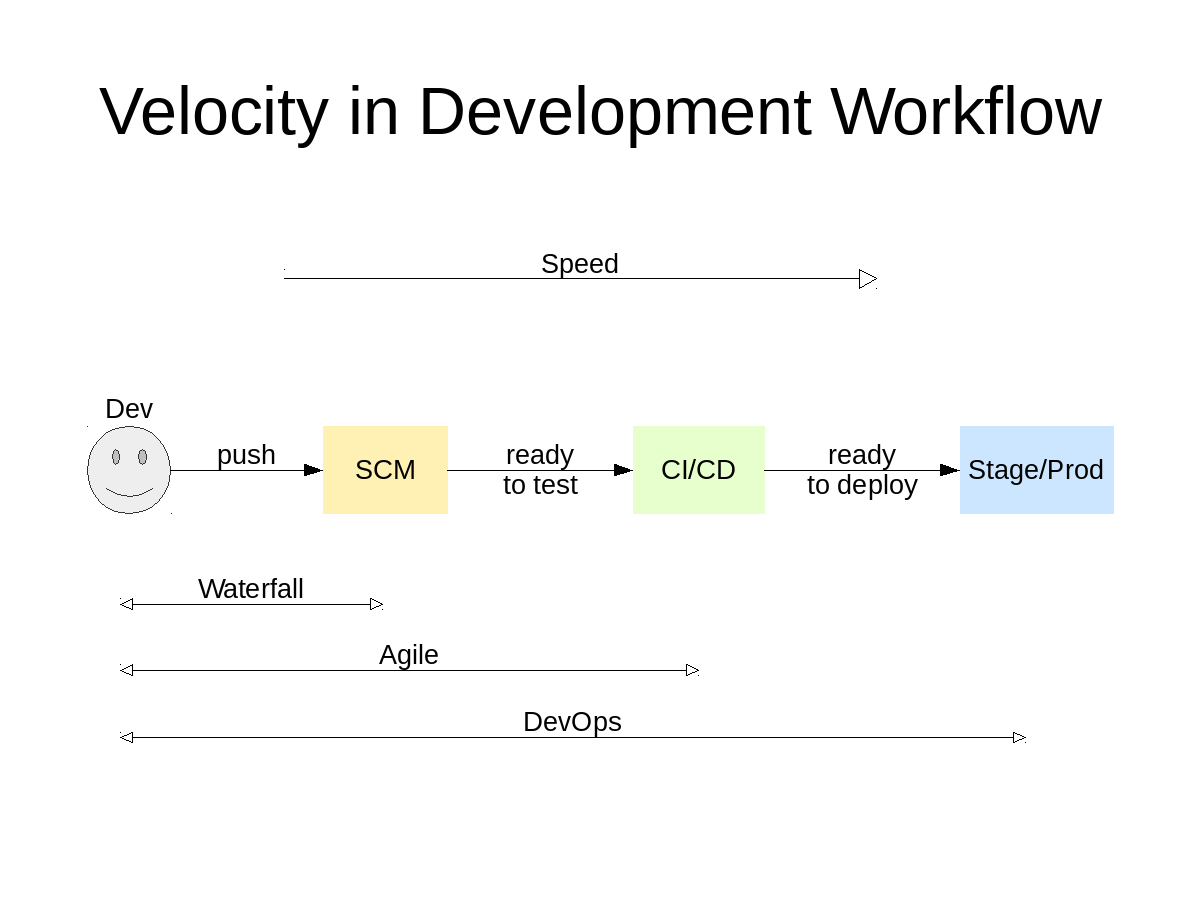
\includegraphics{media/ch2-devops.png}
\caption{Evolution of Development Workflow}
\end{figure}

\section{Scalability in Software
Architecture}\label{scalability-in-software-architecture}

The most common paradigm today is developing \emph{layered} applications
thanks to frameworks, like Django and Rails, that enables developers to
separate the various components, like data, business logic, routing,
templating, caching, etc. This approach has permitted for a better
manageability of spaghetti-code applications since it's possible to find
where is a particular piece of the application and enables scaling
through the layers, usually web/caching, application and database server
components.

While this lead several advantage, with increasing the sizing of
application, it could be to big making hard developing and scaling. The
\emph{microservices} pattern make the modularization another step, and
proposes loosely coupled, but independent applications that communicate
via APIs. This make possible use the best technology (language,
framework, database) for every specific need. Some of them could also be
\emph{stateless}, that does not process data but only

References:

\begin{itemize}
\itemsep1pt\parskip0pt\parsep0pt
\item
  http://microservices.io/articles/scalecube.html
\item
  http://nginx.com/blog/introduction-to-microservices/
\item
  http://martinfowler.com/articles/microservices.html
\item
  http://www.reactivemanifesto.org/
\end{itemize}

\begin{longtable}[c]{@{}llll@{}}
\caption{Summary of Evolution in Software Architecture}\tabularnewline
\toprule
Architecture & Vertical Scaling & Horizontal Scaling & Data partinioning
Scaling\tabularnewline
\midrule
\endfirsthead
\toprule
Architecture & Vertical Scaling & Horizontal Scaling & Data partinioning
Scaling\tabularnewline
\midrule
\endhead
Monolith & yes & no & no\tabularnewline
Layered Monolith & yes & yes & no\tabularnewline
Microservices & yes & yes & yes\tabularnewline
\bottomrule
\end{longtable}

\begin{figure}[htbp]
\centering
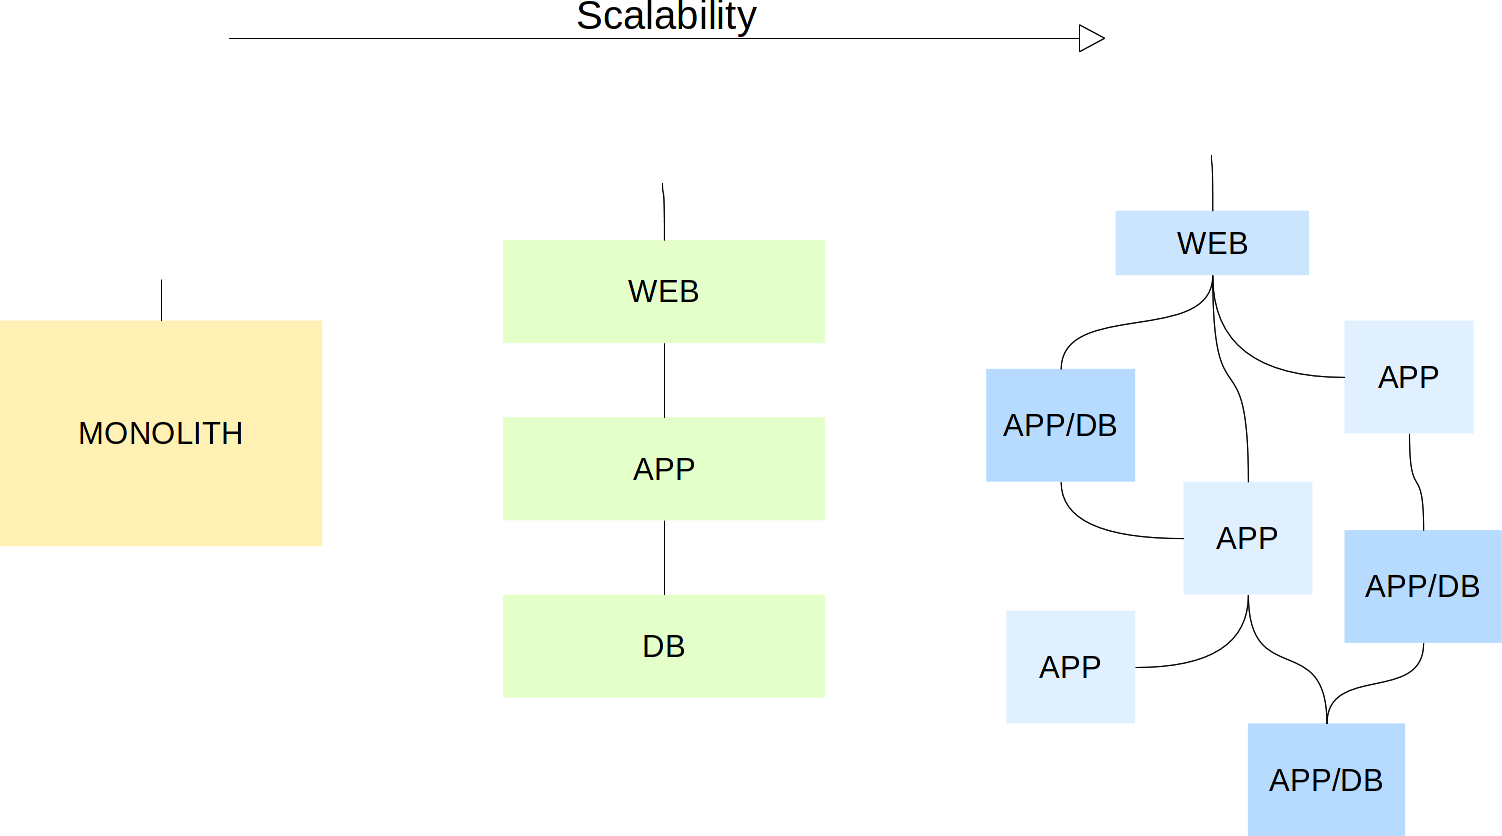
\includegraphics{media/ch2-microservices.png}
\caption{Evolution of Software Architectures}
\end{figure}

\section{Flexibility in Application
Environments}\label{flexibility-in-application-environments}

The final destination of every application is to be deployed somewhere
for producing an added-value for users/customers. Thanks to advantage in
terms of isolation and flexibility than \emph{physical machines}, today
\emph{virtual machines} (VM) represent the atom unit on which
applications are deployed. In fact, working on VMs is logically
equivalent, with a little of overhead.

At the beginning of 2013, was announced Docker, a \emph{container}
runtime (https://www.docker.com/whatisdocker) that aims to be the unit
of launching application components, running reproducible environments,
and concepted for developers friendly via Git-like CLI. Containers
doesn't offer all the isolation of VMs, but reduces the overhead and
permits to optimize resources.

Container technologies already exists, but historically were thinked as
lightweight VMs in order to serve functional-complete operating systems.
Instead, Docker focused on deploying only single processes, separating
the OS from the application layers. Today containers, and Docker in
particular, are in full diffusion and it has been adopted by large
industry.

\begin{longtable}[c]{@{}lll@{}}
\caption{Summary of Evolution in Application
Environments}\tabularnewline
\toprule
Environment & Hardware abstraction & Flexibility\tabularnewline
\midrule
\endfirsthead
\toprule
Environment & Hardware abstraction & Flexibility\tabularnewline
\midrule
\endhead
Physical Machines & no & no\tabularnewline
Virtual Machines & yes & low\tabularnewline
Containers & yes & high\tabularnewline
\bottomrule
\end{longtable}

\begin{figure}[htbp]
\centering
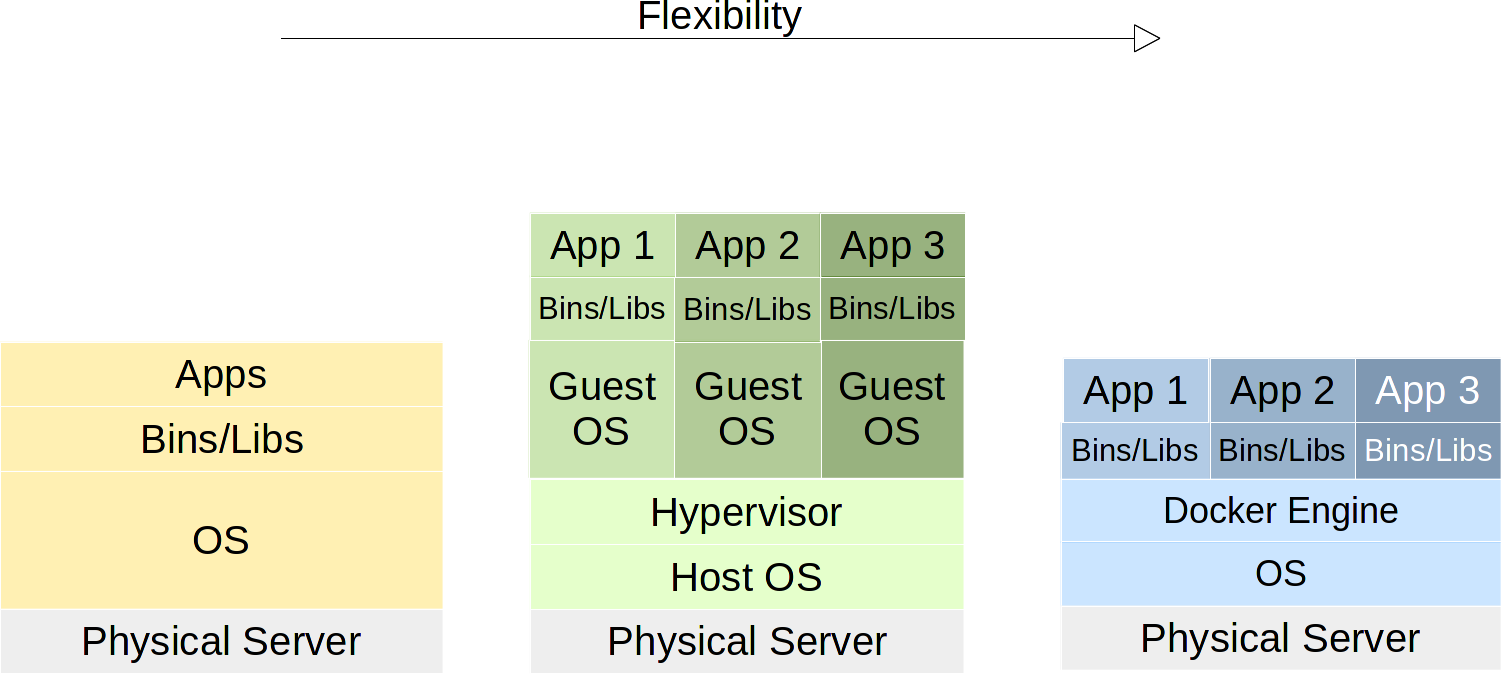
\includegraphics{media/ch2-containers.png}
\caption{Evolution of Application Environments}
\end{figure}

\section{Key Factors: Free Software and Sharing
Economy}\label{key-factors-free-software-and-sharing-economy}

Free Software is based on the following 4 simple principles:

\begin{itemize}
\itemsep1pt\parskip0pt\parsep0pt
\item
  Freedom 0: The freedom to run the program for any purpose.
\item
  Freedom 1: The freedom to study how the program works, and change it
  to make it do what you wish.
\item
  Freedom 2: The freedom to redistribute copies so you can help your
  neighbor.
\item
  Freedom 3: The freedom to improve the program, and release your
  improvements (and modified versions in general) to the public, so that
  the whole community benefits.
\end{itemize}

With Free Software we have the opportunities of:

\begin{itemize}
\itemsep1pt\parskip0pt\parsep0pt
\item
  keep control of software
\item
  learn from design choices and code implementation
\item
  improve the software, with bug-fixing and feature integration
\item
  working on shared projects optimizing costs
\item
  obtain higher quality
\end{itemize}

Free Software enables reuse and leverages the solutions, and enables
rapid feedbacks lowering the \emph{time to release}. In the web/cloud
age, Free Software gained a significant role and is everywhere. It's a
key on which many companies and services rely their trust.

The \emph{Sharing Economy} focuses on relations (a major interaction
between providers and consumers), enhances the community, creates
discussion places, and makes easier direct feedbacks. The Sharing
Economy identifies a collaborative economy, based on cooperation. The
Free Software fits very well in the Sharing Economy for the Information
Technology topics since it avoid lock-in and other restrictive/bad
practices of traditional economy, that aim to centralization instead of
distribution and collaboration.

\section{Case of Study: beFair and Gasista
Felice}\label{case-of-study-befair-and-gasista-felice}

\emph{Gasista Felice} is the main project developed by \emph{beFair}, a
small team involved in the \emph{Free Software} and \emph{Sharing
Economy} networks. beFair is the working environment thanks to which it
has been possible this thesis project.

Gasista Felice is a web platform to manage economy for solidarity-based
purchasing groups (GAS) and suppliers involved in Solidarity-based
economy districts (DES). They all practice Sharing Economy and Social
Business.

The currently production version of Gasista Felice is a web application
built on MVC framework with Python, Django 1.3 and PostgreSQL, with
non-REST APIs and a frontend in JS/jQuery. The work is on a development
version with Python and Django 1.7, PostgreSQL, REST APIs and frontend
in AngularJS and Bootstrap.

\section{A Solution for Current State of
Art}\label{a-solution-for-current-state-of-art}

The following diagram represents a possible summary of the IT evolution
in last decades from multiple point of views:

\begin{longtable}[c]{@{}llll@{}}
\caption{Summary of Evolution in IT}\tabularnewline
\toprule
& 1990's & 2000's & 2010's\tabularnewline
\midrule
\endfirsthead
\toprule
& 1990's & 2000's & 2010's\tabularnewline
\midrule
\endhead
\emph{Development Workflow} & Waterfall & Agile & DevOps\tabularnewline
\emph{IT Operations} & IaaS & IaaS+ & PaaS\tabularnewline
\emph{Software Architecture} & Monolith & Layered Monolith &
Microservices\tabularnewline
\emph{Application Environment} & Physical Machines & Virtual Machines &
Containers\tabularnewline
\bottomrule
\end{longtable}

The solution provided is a Proof of Concept (PoC), thinked beyond
academic purpose for future real use, of a pre-configured free/libre
toolset that enables IT operators to build a PaaS on top of a IaaS/cloud
infrastructure, who aims to be optimal for scaling microservices, and
DevOps-oriented via CD and container as the atomic unit.

Has been follow some guidelines:

\begin{itemize}
\itemsep1pt\parskip0pt\parsep0pt
\item
  elasticity
\item
  lightweight (should not occupy too much resources, compiled languages
  over interpreted/virtualized ones)
\item
  reuse pre-existent components (don't reinvent the wheel)
\item
  reuse pre-existent network layers (avoid dedicated transport layer via
  agents/daemons, to install/configure/manage/update, and more surface
  attack)
\item
  composable pieces with simple interface (composability/pluggability
  over monolith)
\item
  convention over configuration: by default it should works (quite)
  out-of-the-box, but remain customizable (low entry wall)
\item
  automation everywhere possible, few manual commands to install/deploy
\item
  avoid tools requires programming language or custom syntax for
  configuration
\item
  stay on shoulders of giants (avoid too small community and risk to
  adopt tools without a solid/active contributor community)
\item
  minimize external dependencies
\item
  low dependency from IaaS for (future) private cloud
\end{itemize}

There are recent similar projects that should be quoted for
completeness:

\begin{itemize}
\itemsep1pt\parskip0pt\parsep0pt
\item
  \emph{Apollo}\cite{Apollo} from Capgemini, an open-source platform for
  apps, microservices and big data. It consists of Mesos cluster
  provisioning and orchestration using Packer and Terraform
\item
  \emph{MANTL}\cite{MANTL} from Cisco Cloud, formerly
  \emph{Microservices Infrastructure}, is a modern platform for rapidly
  deploying globally distributed services
\end{itemize}

With these goals in mind, the following toolset has been chosen:

\begin{itemize}
\itemsep1pt\parskip0pt\parsep0pt
\item
  Terraform: Infrastructure Provisioning
\item
  Docker Engine: Container Runtime
\item
  CoreOS: GNU/Linux distribution for containers
\item
  Kubernetes: Container Cluster Orchestration
\item
  OpenShift v3: PaaS for modern workflow
\end{itemize}

\begin{figure}[htbp]
\centering
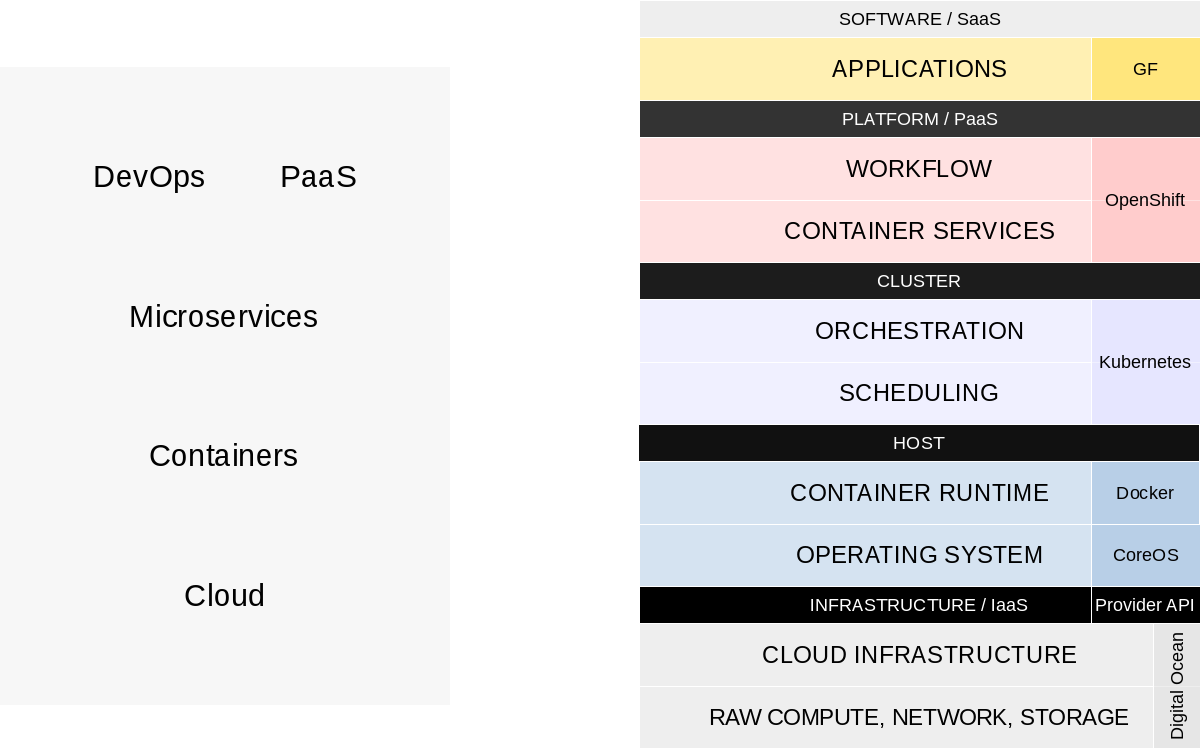
\includegraphics{media/ch2-solution.png}
\caption{From current state of art to a modern solution}
\end{figure}
\chapter{Containerized Applications}\label{containerized-applications}

This chapter introduces containers' core concepts, differences from
previous virtualization and container technologies, and how the use case
application could be containerized.

\section{Container Runtime}\label{container-runtime}

\emph{Docker Engine} was released at the beginning of 2013 from a PaaS
company, as a lightweight alternative to VMs to running and develop
components of applications. Since then, it gained consent by large part
of IT industry and today it's the de-facto standard for container
technologies.

While traditional container technologies like OpenVZ aimed to emulate a
full functional operating system, Docker focused only on running single
processes, separating the application from the OS.

Some of the advantages in using Docker are:

\begin{itemize}
\itemsep1pt\parskip0pt\parsep0pt
\item
  reproducible and standardized environments between development,
  staging, QA and production
\item
  reduce overhead respect to VMs used for deploy single application
\item
  improve isolation and security respect to OS that hosts more
  applications
\end{itemize}

Under the hood, Docker Engine it's composed mainly by a Git-like command
line interface, a daemon and \emph{libcontainer}, a library that use
Linux kernel capabilities such as \emph{namespaces} and \emph{cgroups}.

\begin{figure}[htbp]
\centering
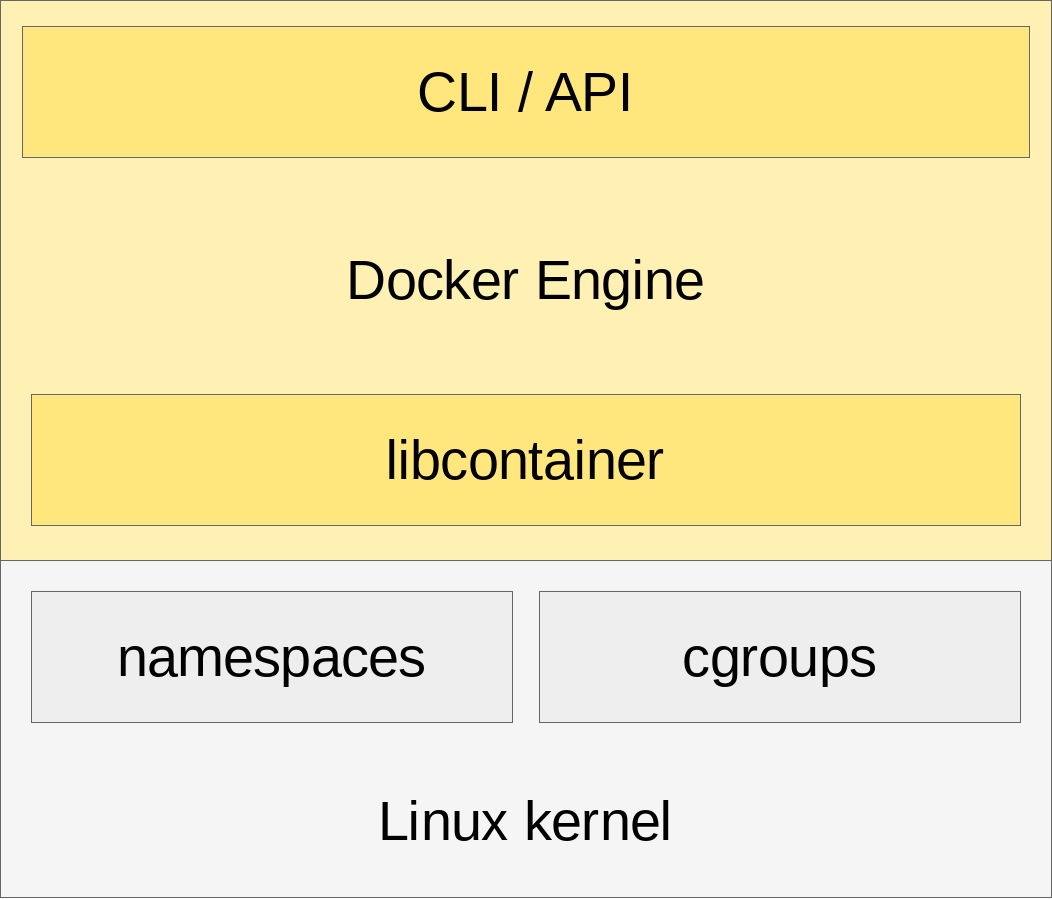
\includegraphics{media/ch3-docker.png}
\caption{Overview of Docker Engine}
\end{figure}

\begin{figure}[htbp]
\centering
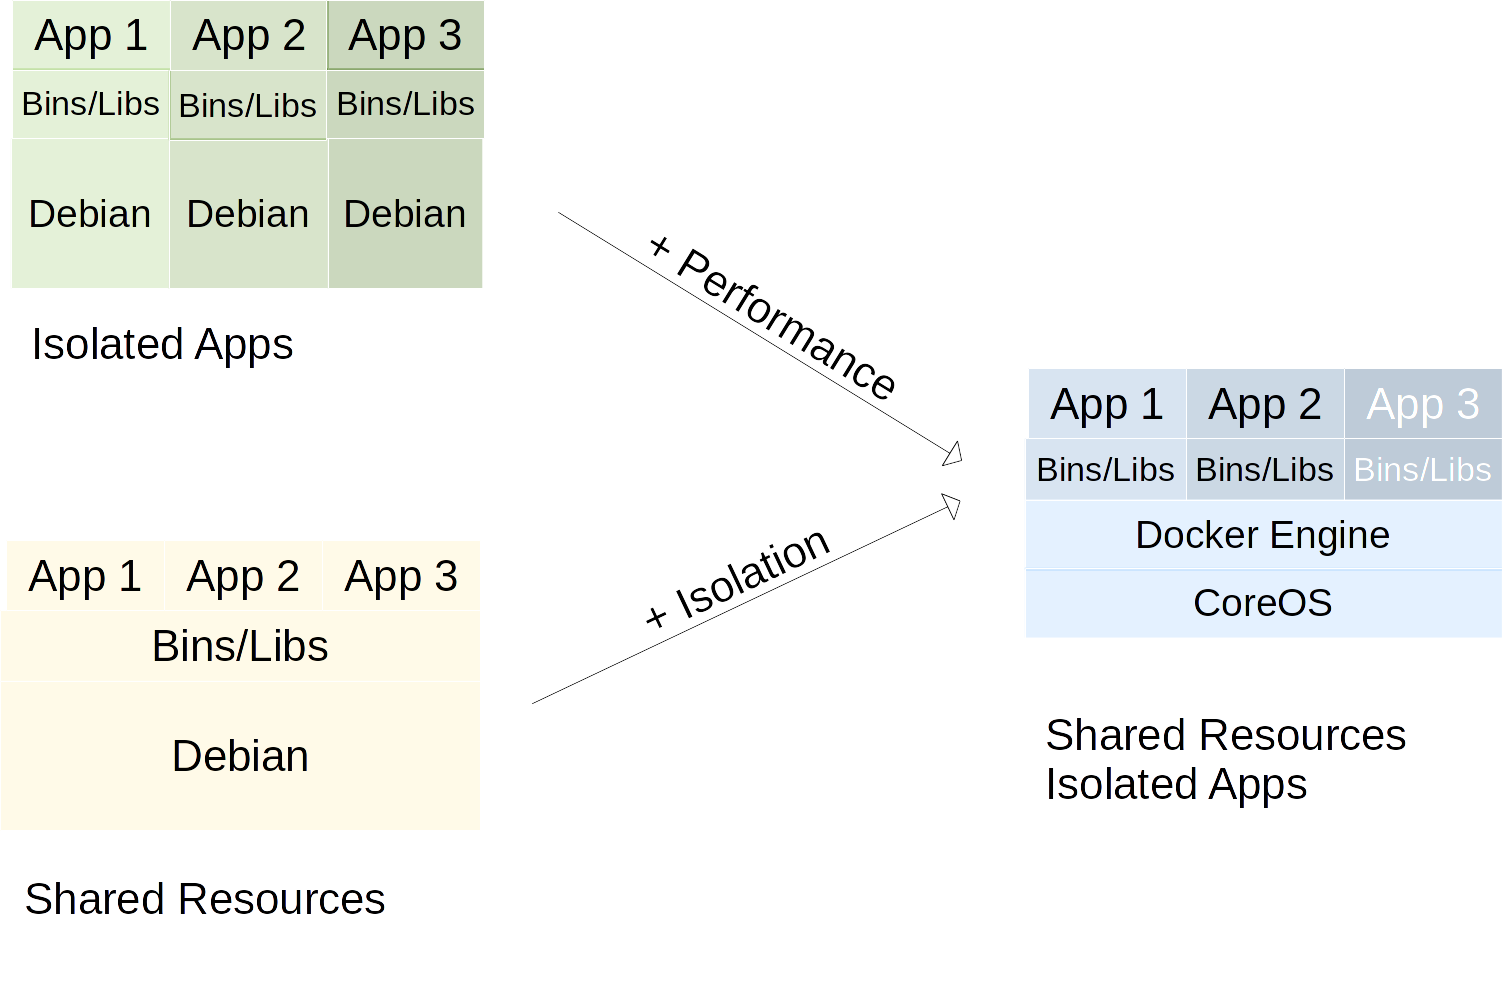
\includegraphics{media/ch3-docker_multiapps.png}
\caption{Performance and Isolation in Multiapps Deployment}
\end{figure}

Someone sees containers more as ``lightweight VMs'', so has been
prepared an alternative base image
(https://github.com/phusion/baseimage-docker). In this case there are a
canonical init dademon as PID 0, instead of the application process
itself. This was particular useful in the early period since it was
needed for some components that depends on specific system feature, such
as syslog, and other purposes. But today Docker includes directly that
kind of features, so this need is decreased.

\begin{itemize}
\itemsep1pt\parskip0pt\parsep0pt
\item
  Part 1
  (http://blog.phusion.nl/2015/01/20/docker-and-the-pid-1-zombie-reaping-problem/)
\item
  Part 2
  (http://blog.phusion.nl/2015/01/20/baseimage-docker-fat-containers-treating-containers-vms/)
\end{itemize}

There are also alternative container runtimes, such as \emph{rkt} (read
``rocket'') (https://github.com/coreos/rocket) that focuses on
reliability and security in production environment.

On June 22, 2015 was announced the \emph{Open Container
Project}\cite{OpenContainerProject} from \emph{Linux Foundation} and
major companies with the target of an industry-wide standard, taking
Docker as the starting point.

\section{Gasista Felice's
Architecture}\label{gasista-felices-architecture}

To apply this to the use case Gasista Felice, the first step is
splitting the application in well-defined components, then containerize
one by one.

In a traditional way, one would have said that the components are
AngularJS for frontend, and Django and PostgreSQL for backend. Instead,
in DevOps-oriented context with dev/prod parity, components should be
the same used in production:

\begin{itemize}
\itemsep1pt\parskip0pt\parsep0pt
\item
  \emph{NGiNX}, web/caching server and reverse proxy
\item
  \emph{harp}, frontend server with built-in preprocessors
\item
  \emph{uWSGI}, web application server
\item
  \emph{PostgreSQL}, relational database
\end{itemize}

In addition, following che \emph{12factor} guidelines, a convention is
to use:

\begin{itemize}
\itemsep1pt\parskip0pt\parsep0pt
\item
  environment variables for configuration
\item
  TCP sockets for inter-container communication
\end{itemize}

So Django settings should be based on \emph{environment variables} with
some defaults. Has been chosen \texttt{APP\_ENV} as main variable that
determines a different behavior of backend. For example, when in
development environment, there is the need of reloading app as soon as
possible with code changes, while in production environment there will
need of more workers and a periodical offloading task.

Another convention is to minimize the mutating components, so the file
system should be read-only by default (including binaries and
libraries), and only well defined directories should be writable
(e.g.~files uploaded by application users).

\section{Container Images}\label{container-images}

As of virtual machines consists of a base disk image and one or more
instances, so containers providers base images and one or more instances
(``real'' containers) running on. In particular, Docker applies the
concept of \emph{Copy on Write} (CoW) that consist of, starting from a
well-defined file system status, write only the differences from it, in
order to minimize the disk usage.

There are base images of common operating system (Debian, Ubuntu,
CentOS) but also language-specific runtimes (Python, NodeJS, Java).
Starting from here it's possible build custom images contains the
application components. In addition, every image has one or more
\emph{tags} in order to provide different versions: e.g.~in
\texttt{debian:8} the \texttt{8} is the tags part that identifies
\emph{Debian Jessie}, but it's also possible define the Debian testing
image with \texttt{debian:9}.

The main way to build Docker images is via \emph{Dockerfiles}, files
that include:

\begin{itemize}
\itemsep1pt\parskip0pt\parsep0pt
\item
  the base image via the \texttt{FROM} directive
\item
  a \texttt{MAINTAINER} reference
\item
  \texttt{ENV}ironment variables declaration
\item
  \texttt{COPY}ing data inside the image
\item
  \texttt{RUN} commands
\item
  TCP ports to expose via \texttt{EXPOSE} directive
\item
  \texttt{CMD} as the default command to run when starting the container
\item
  others as defined in Docker builder reference
  (https://docs.docker.com/reference/builder/)
\end{itemize}

Following the Docker best practices
(https://docs.docker.com/articles/dockerfile\_best-practices/) has been
developed some images as shown in the following picture:

\begin{figure}[htbp]
\centering
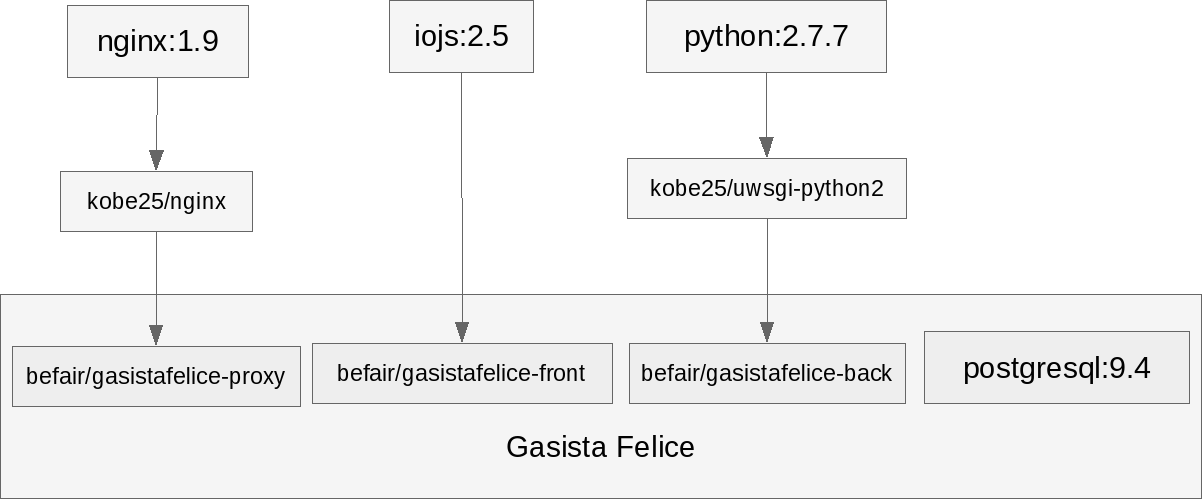
\includegraphics{media/ch3-images_tree.png}
\caption{Container Images Dependency Tree}
\end{figure}

In order to follow the DRY principle, has been developed \texttt{nginx}
and \texttt{uwsgi-python2} base images that provides a common
environment for potential other containerized applications.

The backend of Gasista Felice is an application written in Python with
Django web framework, and served by uWSGI application server. In the
base image has been setted default values for uWSGI, Python, Debian and
PostgreSQL client, were added an \emph{app} Unix user/group and were
installed uWSGI and Python core packages. Note that since uWSGI is the
default process, when a real container will be started, uWSGI take all
the configuration from these defaults and eventual future additions of
overriding.

Then the Dockerfile of Gasista Felice backend, including installation of
dependencies, and copying of application code.

The NGiNX/proxy component also has a base image that move logging to
stdout/stderr and other small customizations.

Instead the Gasista Felice proxy Dockerfile provide a production-ready
configuration, with static files caching.

Another components consist of the Harp server that served static
processed content of frontend. In future this component could be
eliminated, since once the files are generated they could be served
directly from NGiNX.

The PostgreSQL image instead is ready as it is, so it's not be
customized.

\section{Container Orchestration}\label{container-orchestration}

Since an application is splitted in more well-defined components, there
is also the need of a container orchestrator in order to run a multi-container application.

For this target has been chosen \emph{Docker Compose}
(https://docs.docker.com/compose/), a basic tool to deploy applications
in development, similar to Vagrant for VMs. Docker Compose will resolve
the dependency graph of components and linked them together. While
Docker Engine provides the core capabilities, Docker Compose represent
the tool developers use the majority of time.

Following the \href{https://docs.docker.com/compose/yml/}{docker-compose.yml reference}, the containers was orchestrated
(only for develoment) with \emph{Docker Compose}. So running the whole
application is simple as run \texttt{docker-compose\ up} command!

\begin{figure}[htbp]
\centering
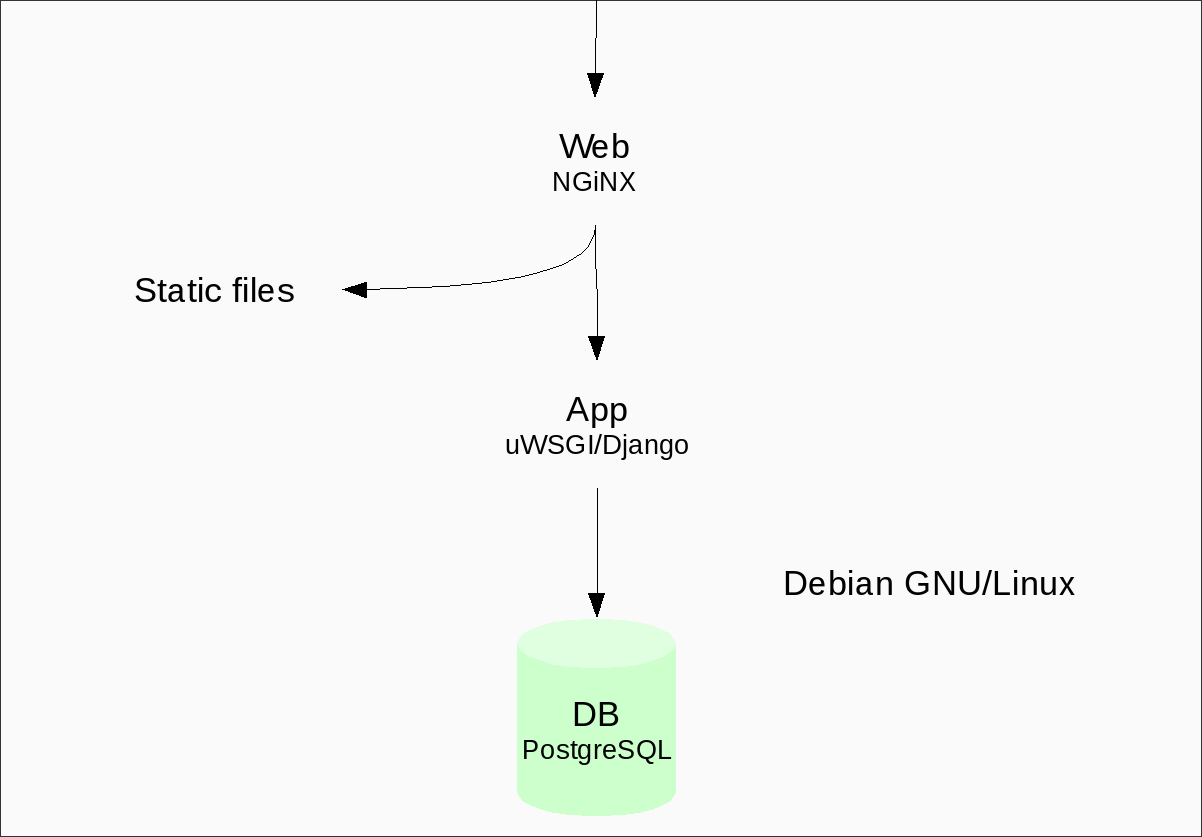
\includegraphics{media/ch3-gf_old.png}
\caption{Gasista Felice before containerization}
\end{figure}

\begin{figure}[htbp]
\centering
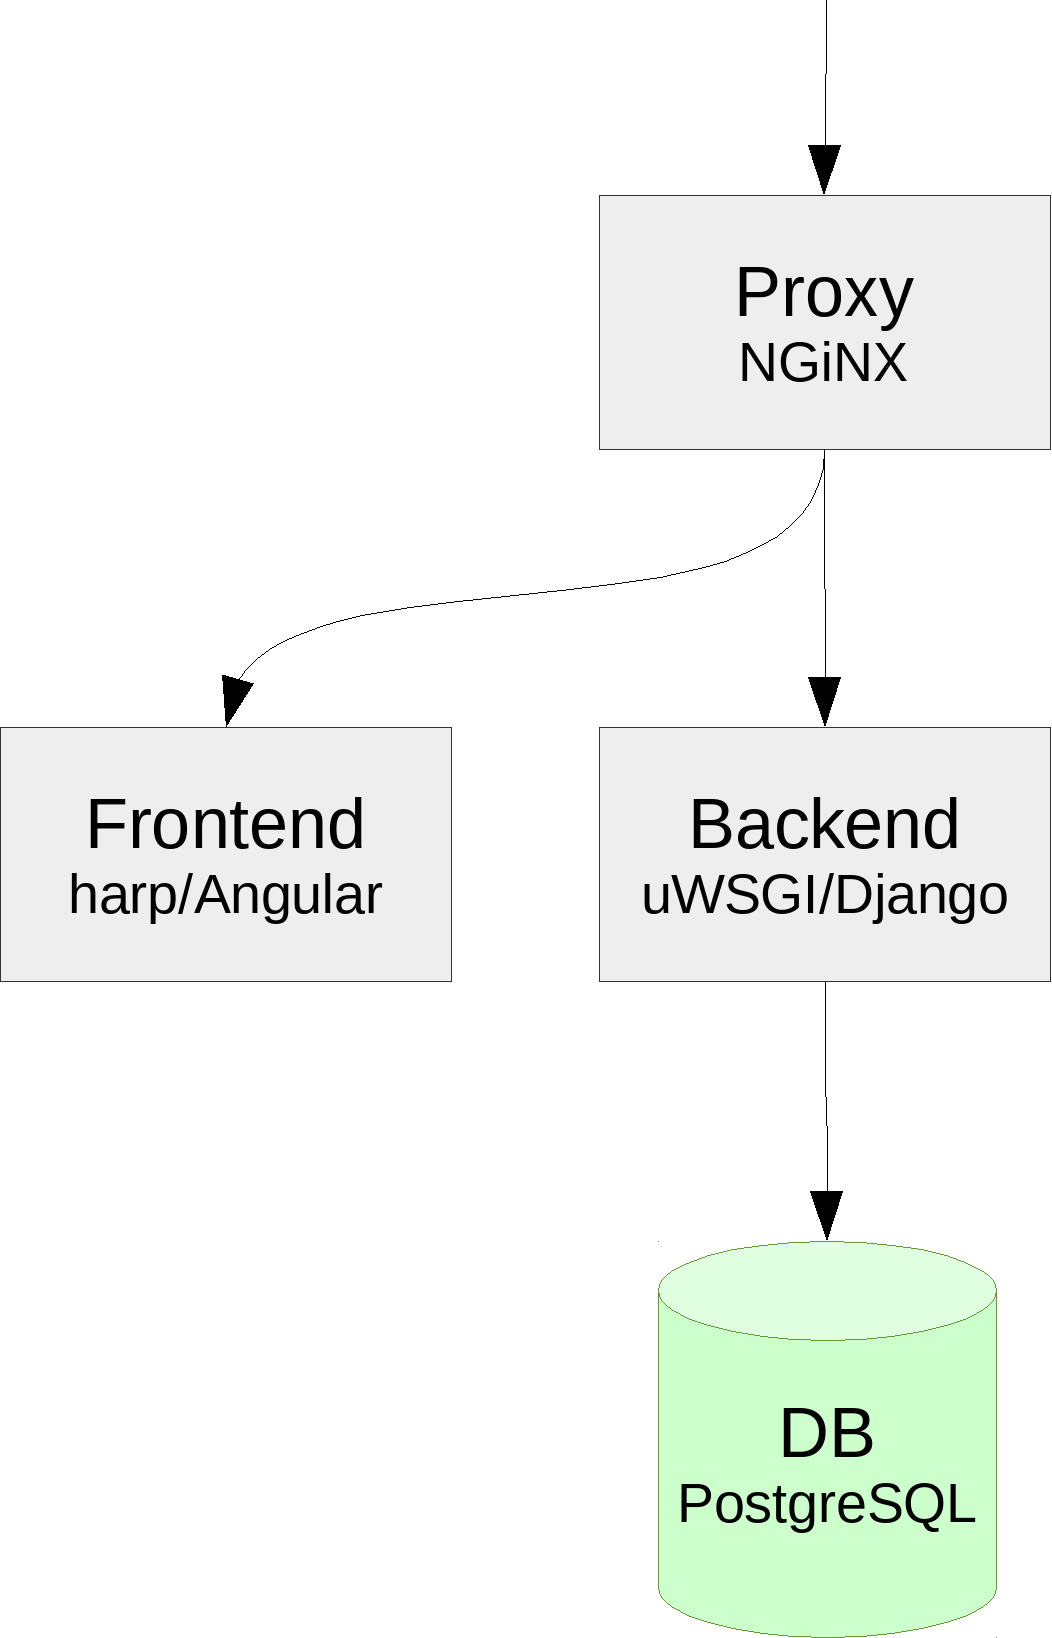
\includegraphics{media/ch3-gf.png}
\caption{Gasista Felice after containerization}
\end{figure}
\chapter{IaaS and PaaS bootstrapping (or Cluster bootstrapping)}\label{iaas-and-paas-bootstrapping}

In order to deploy a containerized application in staging or production, first there is the need of a suitable environment.  While a development environment only need of launching one application with limited usage (only the developer itself) exposing only at localhost, a production environment has much more prerequisites.  The application should be always available, supporting many concurrent users from a public DNS, and lastly many instances of the same application could run at the same time.

This chapter will cover the process of launching the platform (in the PaaS way) on top of an IaaS from a cloud provider, delegating to the next one the internals of this PaaS and how running applications on top of it.

Usually a non trivial production environment is not composed by a unique machine but it's distributed on more hosts collaborate each other to enable further possibilities.  In particular CoreOS, Kubernetes and OpenShift were born with native concept of cluster, in which it's possible classify the hosts in 2 roles:
\begin{itemize}
\item \textit{master} (M), a control host of the life of the whole cluster
\item \textit{node} (N), a worker host on which run applications
\end{itemize}

Then, looking at the possible clustered architectures provided, has been divided 3 kind of possible cluster architectures depends of configuration complexity level:
\begin{itemize}
\item a single host with both master and node roles
\item 1 master and multiple nodes
\item multiple masters and nodes
\end{itemize}

\begin{figure}[htbp]
\centering
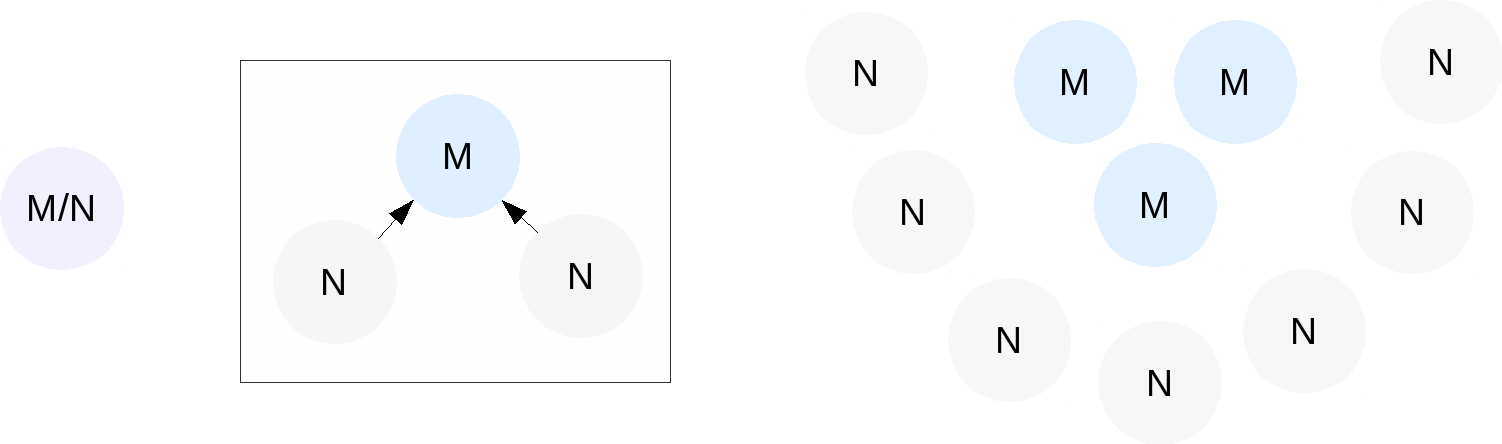
\includegraphics{media/ch4-clusters.png}
\caption{Cluster variants}
\end{figure}

While the first one represents only a very basic limit case, and the last one an advanced configuration for medium to big environments, the second one fits the needs of a small environment, with a balance between roles isolation, low cluster overhead and configuration complexity.  In particular will be used the simplest sub-case with a total of 3 hosts:  1 master and 2 nodes.

\section{IaaS Providers}\label{iaas-providers}

The first step is choice an IaaS provider for machines (compute and storage) and networking.  Even if there is no theoretical need of virtualization, there is a pragmatical one since the resources needed for every host is only a fraction of a whole modern physical server.  It's relevant note that instead of using virtualization for separating applications, in this case it will used for take only a part of the resource of a physical server, and containers represent the level for isolating the applications.  In conclusion, in order to pull up the cluster, there will take 3 VMs from a cloud provider.

In summary, the needed features of the cloud provider are:
\begin{itemize}
\item CoreOS native support, with additional possibility of customizing images
\item integration with existing tools (\textit{Terraform} in particular)
\item simple plans avoiding proprietary or provider-specific services
\item relatively economic
\end{itemize}

Then will be useful some cluster-oriented features like:
\begin{itemize}
\item private network
\item low-cost for intra-cluster traffic
\end{itemize}

In additional extra features could be the integration of DNS Management in order to cover all the infrastructure-level services.

\textit{Digital Ocean} (DO), built on top of free software \textit{QEMU} and \textit{KVM}, matches all the above points.

The master host doesn't run applications, and its sizing depends on number of nodes and containers to manage, while the sizing of nodes depends on  resources needed for applications.  After looking at Digital Ocean offer, the following plans were chosen:

\begin{itemize}
\item 1 master with 1 core, 1GB memory and 30GB SSD
\item 2 nodes with 2 cores, 2GB memory and 40GB SSD each one
\end{itemize}

For a total of 5 cores, 5GB memory and 110GB SSD.  Finally, the cluster has to be composed by hosts in the same data center in order to keeping the latency in intra-cluster communication as low as possible.

\section{Provisioning of IaaS}\label{provisioning-of-iaas}

Using a PaaS means a lot of automation and good practices applied in deploying applications.  For keeping a similar level of automation in provisioning all the lower stack than applications, there is need of additional tools.

In particular the tasks should be:
\begin{itemize}
\item describe the resource of infrastructure, possibly in a declarative way
\item resolve the dependencies graph of infrastructure resources
\item communicate with the provider through APIs (and auth token) doing the necessary operations
\item connecting via SSH to the hosts for bootstrapping
\item setting up the public DNS in order to point to a specific node of the cluster
\end{itemize}

\textit{Ansible} and \textit{SaltStack} are popular choices today since includes several modules for lower-level operations (cloud provisioning) but also higher-level ones (application deployment and configuration management).  Since the applications are managed entirely by the PaaS as will be shown in next chapter, these tools are over sized.

\textit{Terraform} (https://terraform.io/) is a more minimal CLI-based tool, focuses only on cloud infrastructure provisioning on which results more productive and powerful.  Terraform apply the changes based on:
\begin{itemize}
\item actual state:  description of current resource states
\item desired state:  description of resource states
\end{itemize}

With these in mind, Terraform process the data doing necessary operations aiming to keep from "actual state" to "desired state".  A basic example could be:
\begin{itemize}
\item actual state:  there is no machines
\item desired state:  there is need of 3 machines
\end{itemize}

So Terraform will communicate to provider via APIs in order to pull up 3 machines, then after the creation of these machines, their data (public IP, etc) will be stored as "actual state".  Then, if there is no need of a VMs, it's only necessary change the desired state and re-apply Terraform.

This approach of Terraform enables the possibility of so-called \textit{Infrastructure as Code} (IaC), that consists in versioning this files contains the states in order to tracks the infrastructure evolution, just as it is a common software project.  This represent a more structured, deterministic and reproducible way to infrastructure management.

In addition, Terraform could be used for enabling powerful features like horizontal host-level auto-scaling, varying the cardinality of the cluster in response to global load changes.

\begin{figure}[htbp]
\centering
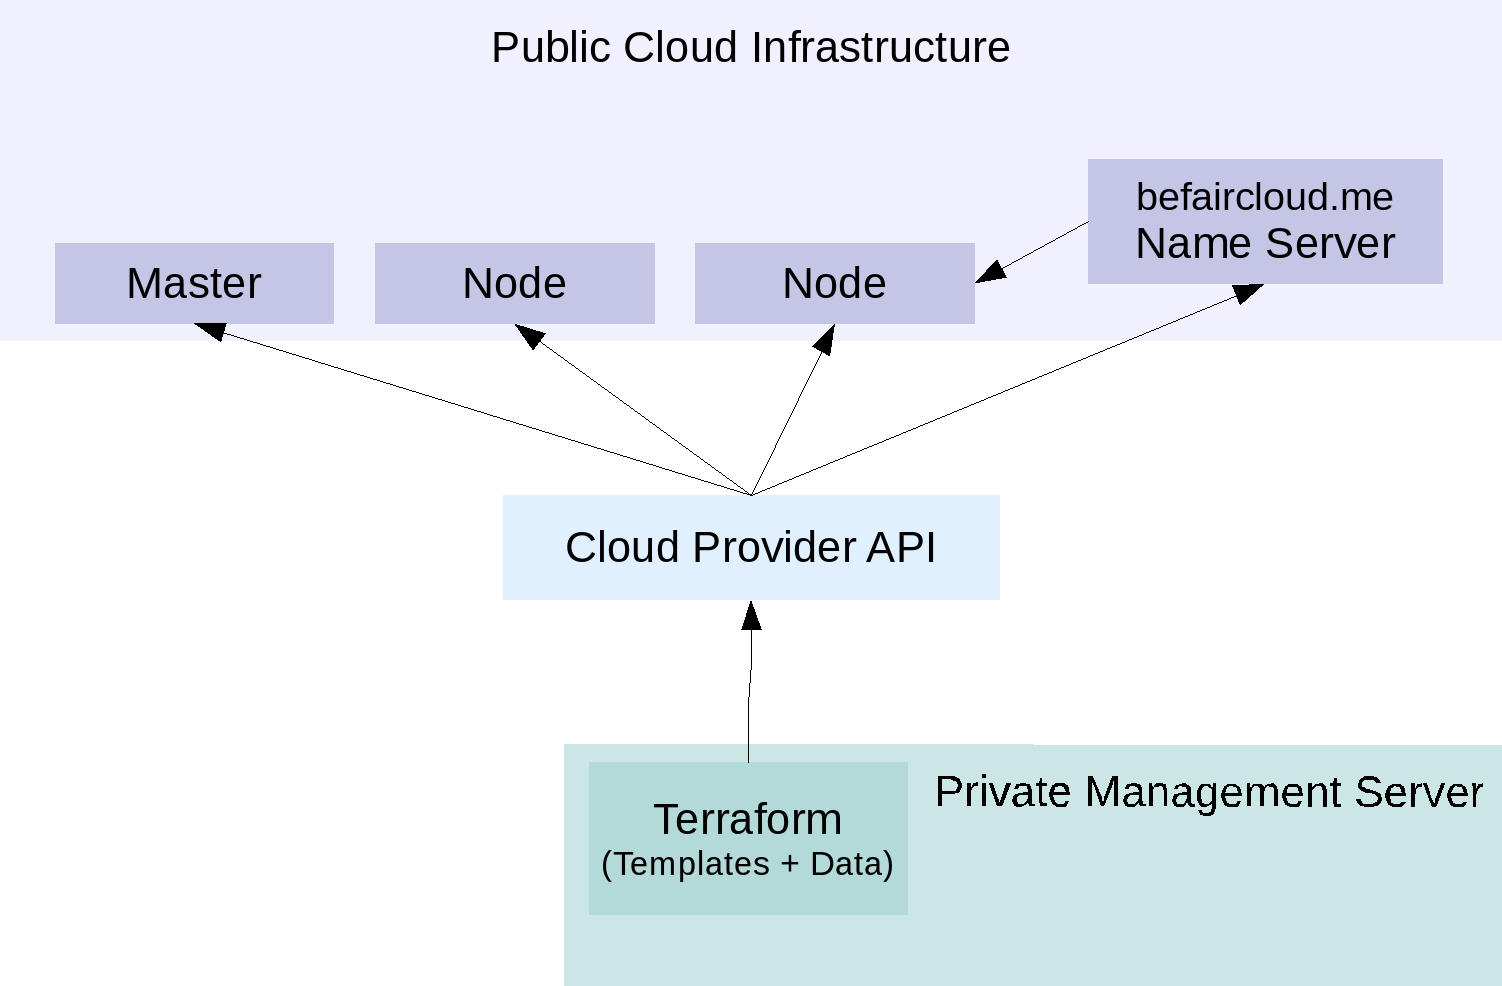
\includegraphics{media/ch4-terraform.png}
\caption{Infrastructure Provisioning with Terraform}
\end{figure}

The resources (in execution order) are:
\begin{enumerate}
\item access token for Digital Ocean APIs (previously generated by provider Web UI)
\item upload temporary public SSH key (used for connection to hosts)
\item PaaS bootstrapping, regarding VMs and configuration (will be covered in the next sub-chapter)
\item DNS management for \textit{befaircloud.me}, a dedicated domain for this project, through Digital Ocean DNS service
\item pointing \textit{*.befaircloud.me} A-type record to the first node
\end{enumerate}

In addition, some variables for parametrization are used for a more DRY configuration.

\begin{figure}[htbp]
\centering
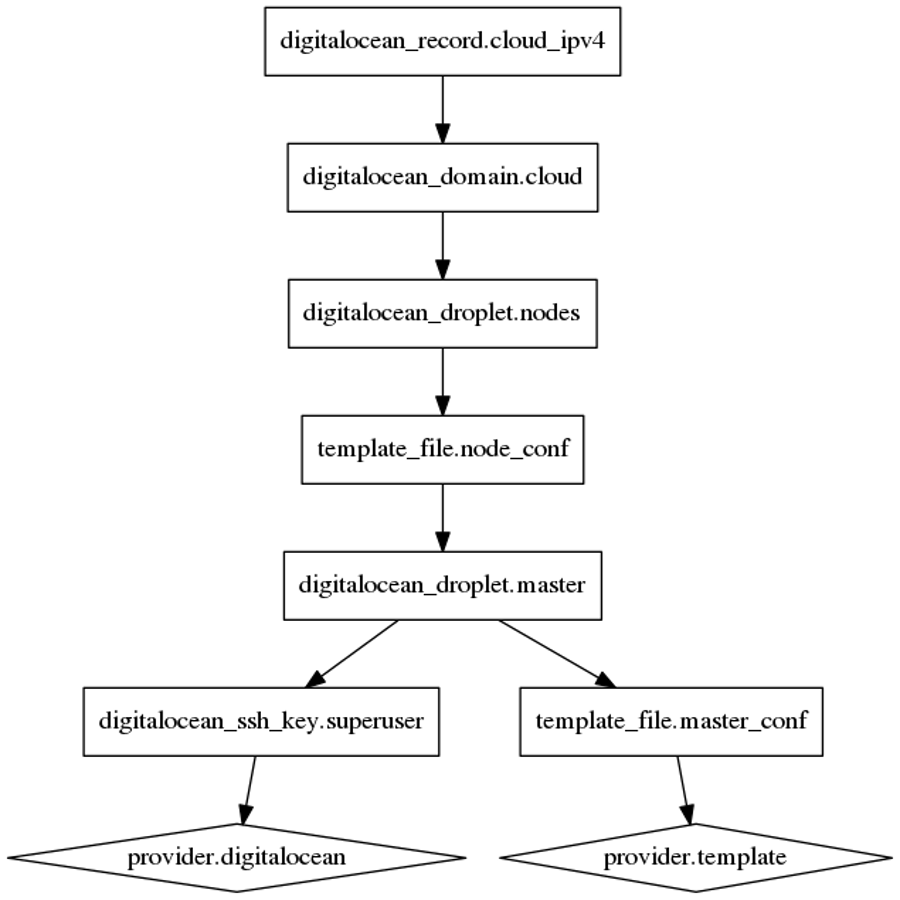
\includegraphics{media/ch4-graph.png}
\caption{Infrastructure Dependency Graph}
\end{figure}

All the Terraform configuration could be seen in the Appendix B.  Note that while Terraform supports custom language, the \textit{Hashicorp Configuration Language} (HCL) and JSON, the choice is to use a standardized, human-readable and clean YAML.

For launching all the infrastructure, it's so simple as running \texttt{make up}, that will do the following tasks:
\begin{enumerate}
\item cleaning previous temporary files
\item compile YAML configurations into JSON
\item creating a temporary SSH RSA 4096bit public/private key
\item create an archive with necessary binaries and configuration files to upload on all hosts
\item launching Terraform's \texttt{plan} in order to plans the operations to do
\item launching Terraform's \texttt{apply} in order to apply the planned operations
\end{enumerate}

At the end, there is some output with commands for complete the bootstrapping and log via SSH to master.

\begin{verbatim}
Outputs:

  step1 = scp -r -i .cache/id -o StrictHostKeyChecking=no core@46.101.133.104:./master .cache/; \
scp -r -i .cache/id -o StrictHostKeyChecking=no .cache/master core@46.101.138.191:./; \
scp -r -i .cache/id -o StrictHostKeyChecking=no .cache/master core@46.101.200.100:./

  step2 = log to master -- ssh -i .cache/id -o StrictHostKeyChecking=no core@46.101.133.104
log to node-0 -- ssh -i .cache/id -o StrictHostKeyChecking=no core@46.101.138.191
log to node-1 -- ssh -i .cache/id -o StrictHostKeyChecking=no core@46.101.200.100
dashboard -- https://46.101.133.104:8443
entrypoint -- http://befaircloud.me
\end{verbatim}

Now the whole cluster is up and running!

For deleting all resources (from VMs to DNS records), it's needed running \texttt{make destroy} that consists of:
\begin{enumerate}
\item \texttt{terraform plan -destroy} for planning deletion of all resources
\item \texttt{terraform destroy} for deleting the planned destruction
\end{enumerate}

\section{Provisioning of PaaS}\label{provisioning-of-paas}

Another core aspect to cover regards the PaaS bootstrapping, the process from vanilla CoreOS to a complete functioning clustered PaaS running Kubernetes and OpenShift.  There internals of cluster is so postponed to the next chapter.

The key technologies used is a combination of Terraform's template feature and \textit{Cloud Config}, an emerging standard for operating system configuration at boot time via a declarative way.  Cloud Config consists of a simple YAML file that an OS (CoreOS, Ubuntu, etc.) could read, with information about hostname, ssh keys and user permissions, files and other settings.  CoreOS added additional features for SystemD units and cluster upgrade.

Since master and node have a different configuration needs, there are been developed two templates.  Terraform use these templates and passing them when requesting the machines. The main dependency is provide the master private IPv4 address to nodes, so they can connect to the master.

The detailed steps for provisioning a master are:
\begin{enumerate}
\item Terraform resolves the Cloud Config template of master and resolves variables in the form \$\{VAR\_NAME\}
\item Terraform calls the API to pull up a new VM with vanilla CoreOS, passing the Cloud Config master, and uploading an archive (with necessary binaries and OpenShift configurations)
\item Digital Ocean parses this template replacing \$public\_ipv4 and \$private\_ipv4 variables
\item Digital Ocean pulls up the master passing Cloud Config template to CoreOS
\item CoreOS reads the full-rendered Cloud Config template, and apply the described configurations
\end{enumerate}

Once the master has been correctly deployed, the nodes could be deployed:
\begin{enumerate}
\item Terraform resolves the Cloud Config template of node, passing the \textit{master IP}.  So this template could be used for every node for that specific master
\item the same steps as for the master
\end{enumerate}

The configuration described in Cloud Config is necessary for:
\begin{itemize}
\item enable SSH login to \texttt{core} user with provided key
\item provide a SystemD unit for bootstrapping the host and write the OpenShift/Kubernetes configuration (different between master and node)
\item provide a SystemD unit for running the main OpenShift/Kubernetes binary (different between master and node)
\end{itemize}

Thanks to this capabilities, this entire process is (quite) totally automated, except for a single command, that is anyway automatically provided by Terraform at the end.

\begin{figure}[htbp]
\centering
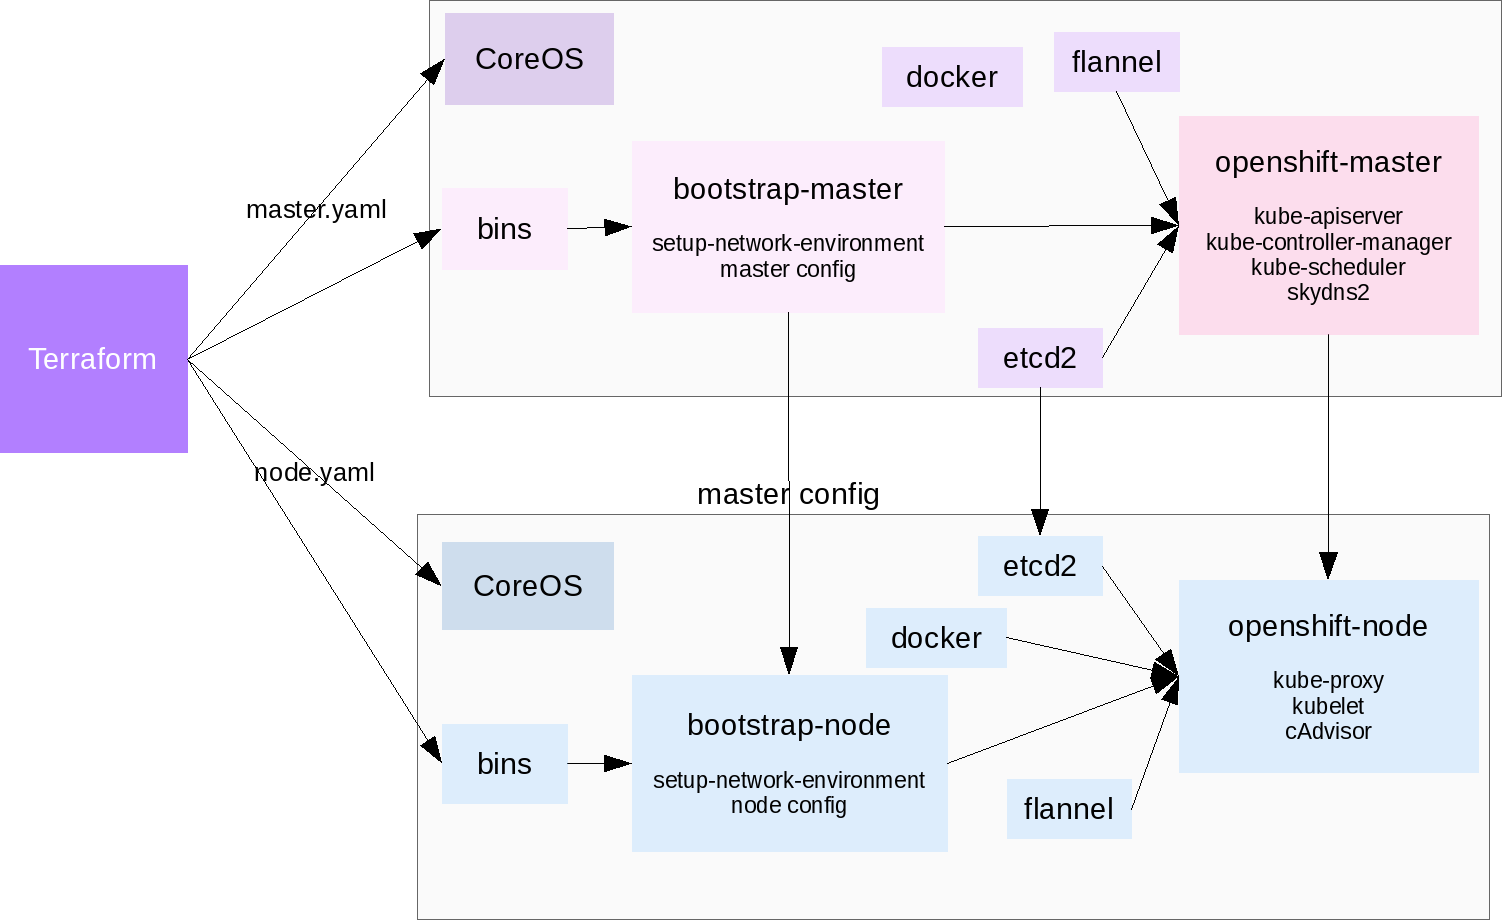
\includegraphics{media/ch4-bootstrap.png}
\caption{Provisioning of the PaaS}
\end{figure}
\chapter{PaaS Management}\label{paas-management}

This chapter describes the stack around a container-based production
environment, and how applications could take advantage on it.

\begin{figure}[htbp]
\centering
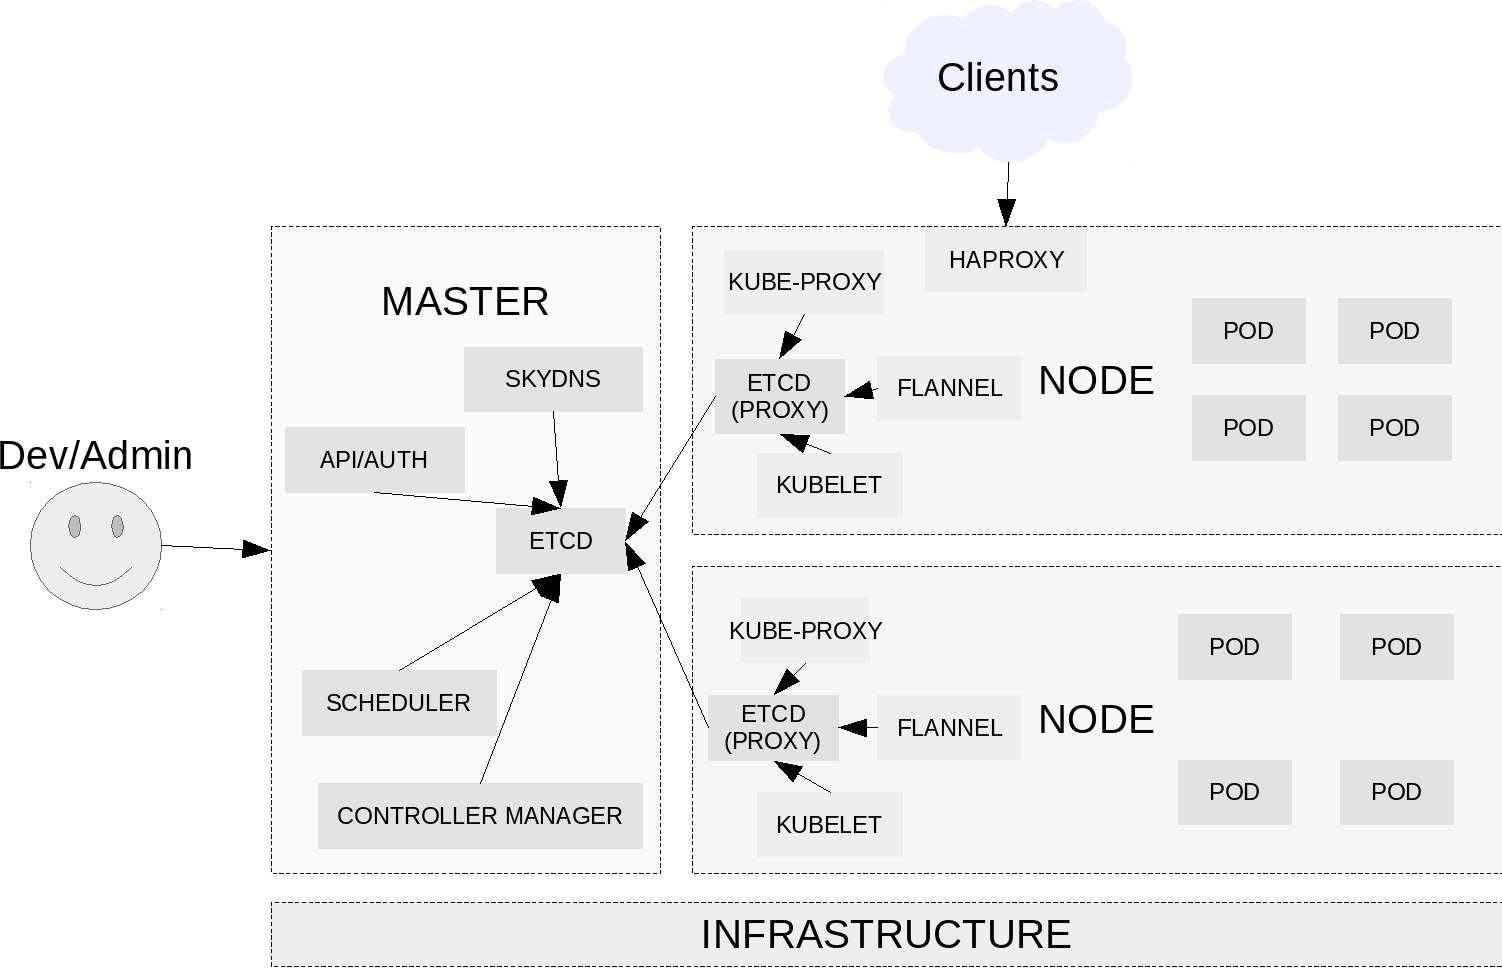
\includegraphics{media/ch5-overview.png}
\caption{Cluster Overview}
\end{figure}

\section{The Container Cluster's
Core}\label{the-container-clusters-core}

The basic building block for deploying containerized application remain
the operating system. But as all the application dependencies are
demanded to containers, there is only need basic functionality, without
package manager and other features of a traditional OS.

\emph{CoreOS} was announced in summer 2013 as a Gentoo-based GNU/Linux
distribution for deploying containers in a clustered environment. CoreOS
occupies few memory and comes with \emph{SystemD}, \emph{Docker} and
tools for distributed cluster environments.

\emph{SystemD} is the de-facto standard in GNU/Linux distribution as
init daemon. It made easy to daemonize processes and has advanced
features such as parallelization and socket activation, so the SSH
daemon is stopped by default, and it will be started only after an
incoming request, in order to save memory.

\emph{Etcd} is a distributed key-value database which represent the core
of the cluster since it has been used for inter-host communication by
all components. It could be used as master-slave (as in this project) or
also in high availability with a simply Raft-based algorithm for master
election. Etcd is the \emph{cluster database}, so it's really a core
component.

\emph{Fleet} provides a distributed init system, extending SystemD
functionality from host-level to cluster-level. This component has not
been used but it's useful for bootstrap the above stack, since it could
deploy SystemD services in all connected hosts.

\emph{Flannel} has been development for providing a subnet mask to every
host, enabling an overlay network for container inter-host
communication. It's a requisites of Kubernetes networking model. At the
boot, Flannel set the network data into etcd under \texttt{/coreos.io}
key.

CoreOS development is organized in 3 channels: alpha, beta and stable.
Alpha is generally release once a week and includes new software, while
stable it's more suitable for production.

Alternatives are Rancher OS (http://rancher.com/rancher-os/), Atomic
(http://www.projectatomic.io/) by Red Hat and Ubuntu Snappy
(http://www.ubuntu.com/cloud/tools/snappy) by Canonical.

\section{Microservices Scaling and
Orchestration}\label{microservices-scaling-and-orchestration}

Kubernetes (http://kubernetes.io/) has been announced at Google I/O in
June 2014, it's a cluster management system, a framework for container
scheduling and orchestration in a clustered environment. It fits a level
on top of an operating system like CoreOS.

Kubernetes has been developed by the same engineers developed the actual
Google infrastructure, and take advantace of that experience.

Core concepts of Kubernetes are:

\begin{itemize}
\itemsep1pt\parskip0pt\parsep0pt
\item
  \texttt{node} is a single node of the cluster
\item
  \texttt{pod} is a set of one or more containers, thinked as a single
  logic unit
\item
  \texttt{replicationController} is concerned about guarantee the
  correct numbers of replicas of a pod
\item
  \texttt{service} provides a virtual IP that load balance to a set of
  pods
\end{itemize}

\begin{figure}[htbp]
\centering
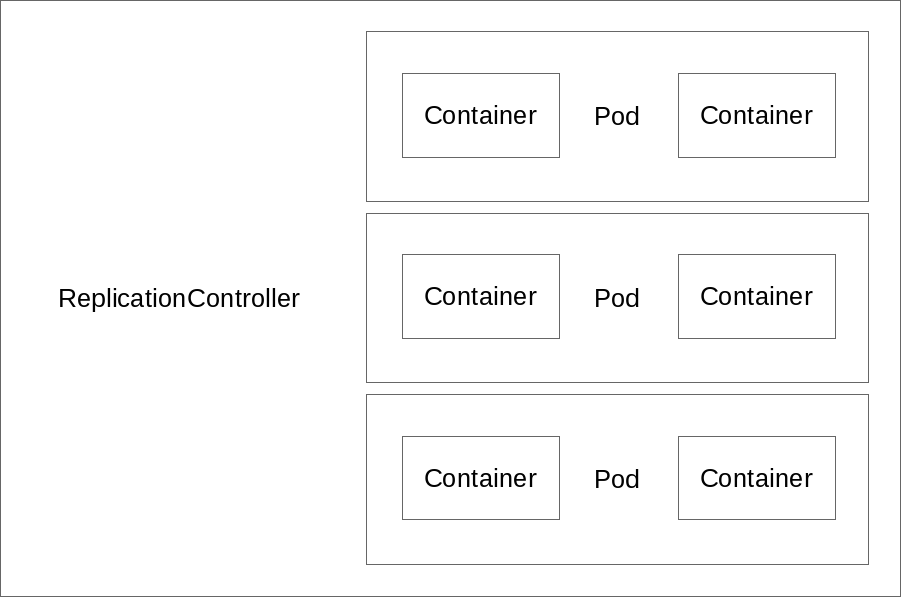
\includegraphics{media/ch5-pods-rcs.png}
\caption{Pods and Replication Controllers}
\end{figure}

\begin{figure}[htbp]
\centering
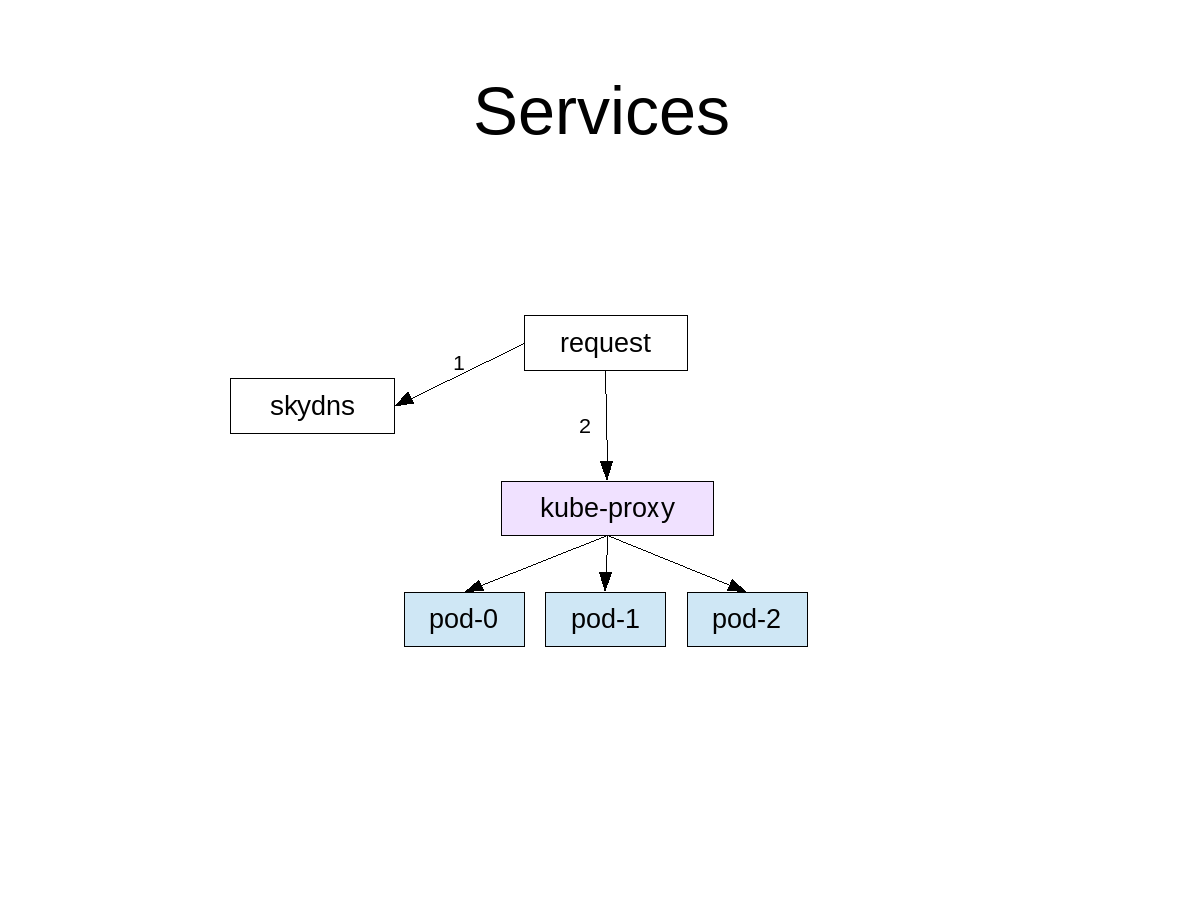
\includegraphics{media/ch5-services.png}
\caption{Scaling Pods with Kubernetes services}
\end{figure}

Components of Kubernetes are divided in master and node. The Master ones
are:

\begin{itemize}
\itemsep1pt\parskip0pt\parsep0pt
\item
  \emph{API Server} validates and configures the data for pods,
  services, and replication contorllers
\item
  \emph{Controller Manager} watches etcd for changes to replication
  controller and then uses the API to enforce the desired state
\item
  \emph{Scheduler} schedule the pods into nodes
\end{itemize}

Instead the components of Kubernetes Node are:

\begin{itemize}
\itemsep1pt\parskip0pt\parsep0pt
\item
  \emph{Kubelet} updates the node as specified in local etcd
\item
  \emph{Proxy} manages the services defined in the API on that node
\end{itemize}

Kubernetes stores the data about \texttt{node}s, \texttt{pod}s,
\texttt{replicationController}s, \texttt{service}s and other objects in
etcd under \texttt{/kubernetes.io} key.

These concepts could be summarized in the following diagram:

\begin{figure}[htbp]
\centering
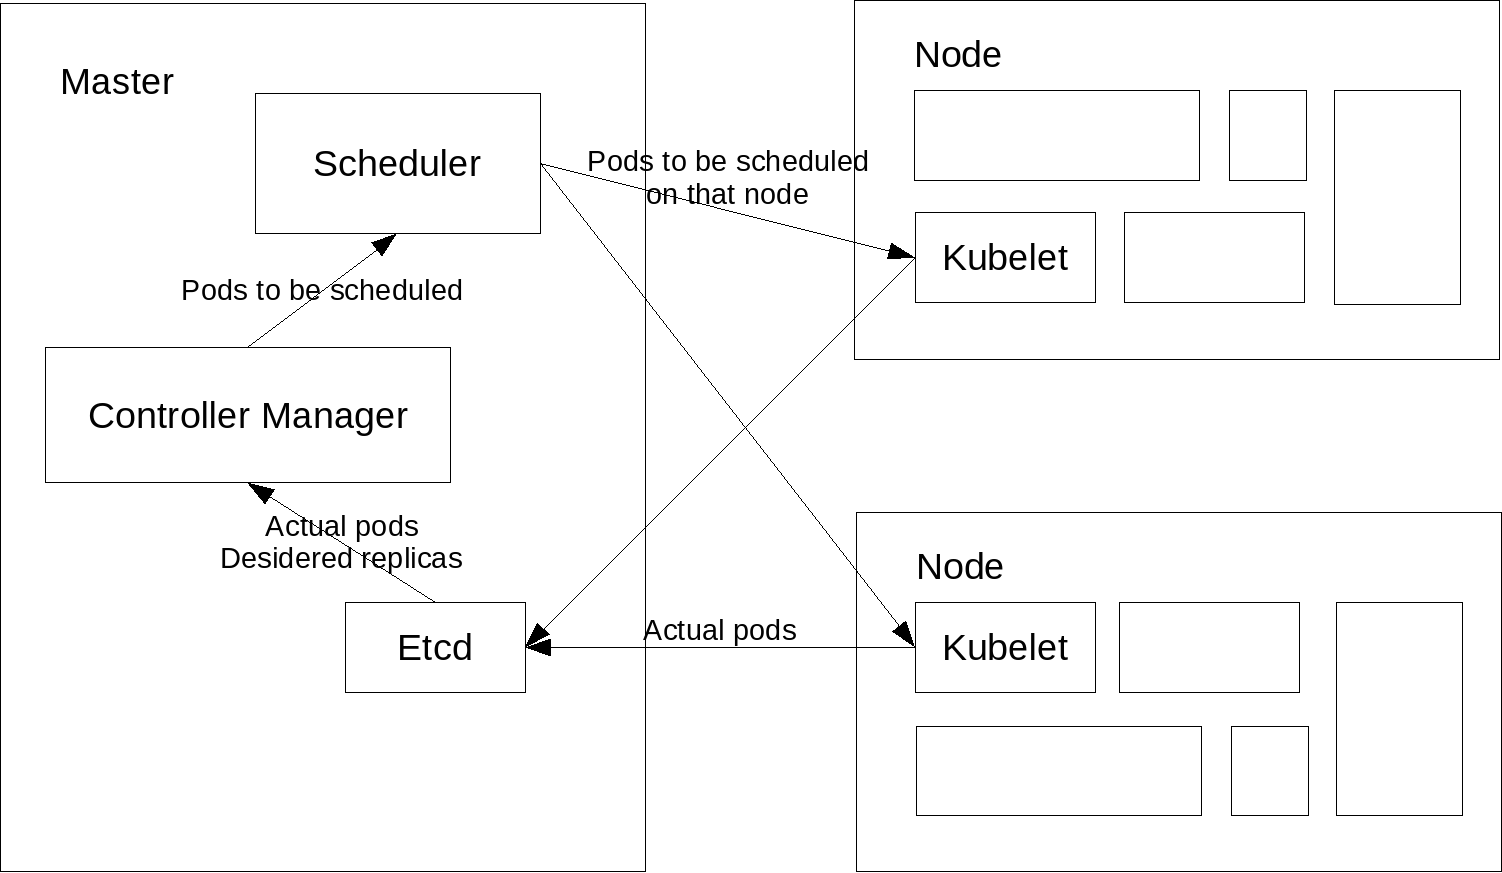
\includegraphics{media/ch5-scheduling.png}
\caption{Replicas and Scheduling}
\end{figure}

On July 20, 2015 the \emph{Linux Foundation} announced the \emph{Cloud
Native Computing Foundation}\cite{CloudNativeComputingFoundation} in
order to standardize the orchestration of components in a cloud
environment, taking Kubernetes as a starting point.

\section{PaaS for Deploying
Applications}\label{paas-for-deploying-applications}

Kubernetes is a great solution, but lacks the concept of application and
the development workflow, so it's more a tool for system specialists. In
order to reach a PaaS abstration, there is needed another level on top
of Kubernetes.

The 3rd version of \emph{OpenShift} is a PaaS built on top of
Kubernetes, providing a solutions for DevOps workflow in modern
container and microservices world.

First of all, OpenShift comes with built-in external router, based on
HAProxy\cite{HAProxy}:

\begin{quote}
HAProxy is a free, open source high availability solution, providing
load balancing and proxying for TCP and HTTP-based applications by
spreading requests across multiple servers. It is written in C and has a
reputation for being fast and efficient (in terms of processor and
memory usage).

HAProxy is used by a number of high-profile websites including GitHub,
Bitbucket, Stack Overflow, Reddit, Tumblr, and Twitter and is used in
the OpsWorks product from Amazon Web Services.
\end{quote}

In order to responding to DNS queries for services, OpenShift includes
\emph{skydns} server.

OpenShift extends Kubernets APIs with additional objects:

\begin{itemize}
\itemsep1pt\parskip0pt\parsep0pt
\item
  \texttt{template} is the building block for applications. Since
  Kubernetes has only conpect of services and not of application,
  template provides a way to define an application as a set components,
  as happens in Docker Compose
\item
  \texttt{route} is configure the HAProxy-based external \texttt{router}
  for external reachability, and point to a \texttt{service}.
\end{itemize}

Future Development will include the following objects in order to enable
Continuous Delivery:

\begin{itemize}
\itemsep1pt\parskip0pt\parsep0pt
\item
  \texttt{build} is the process of creating Docker images from scratch
  or other images
\item
  \texttt{imageStream} represent an image storaged in a repository
\item
  \texttt{deploymentConfig} extends \texttt{replicationController}
  enabling rolling updates in response to signals
\end{itemize}

OpenShift stores the own objects in etcd under \texttt{/openshift.io}
key.

These concepts could be summarized in the following diagram:

\begin{figure}[htbp]
\centering
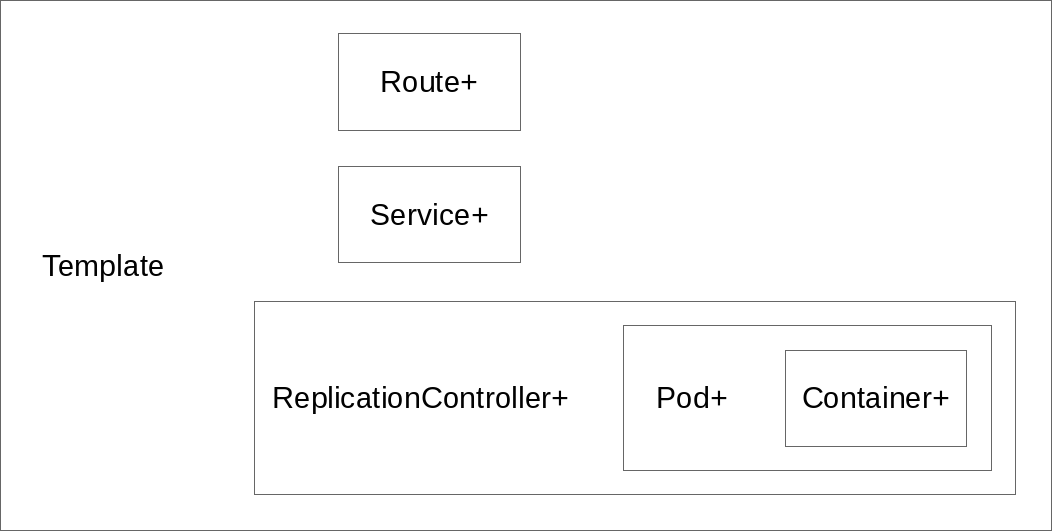
\includegraphics{media/ch5-template.png}
\caption{Route and Template objects}
\end{figure}

Gasista Felice consist of a \texttt{template} that includes a
\texttt{replicationController}/\texttt{service} for every container,
plus a \texttt{route}.

\begin{figure}[htbp]
\centering
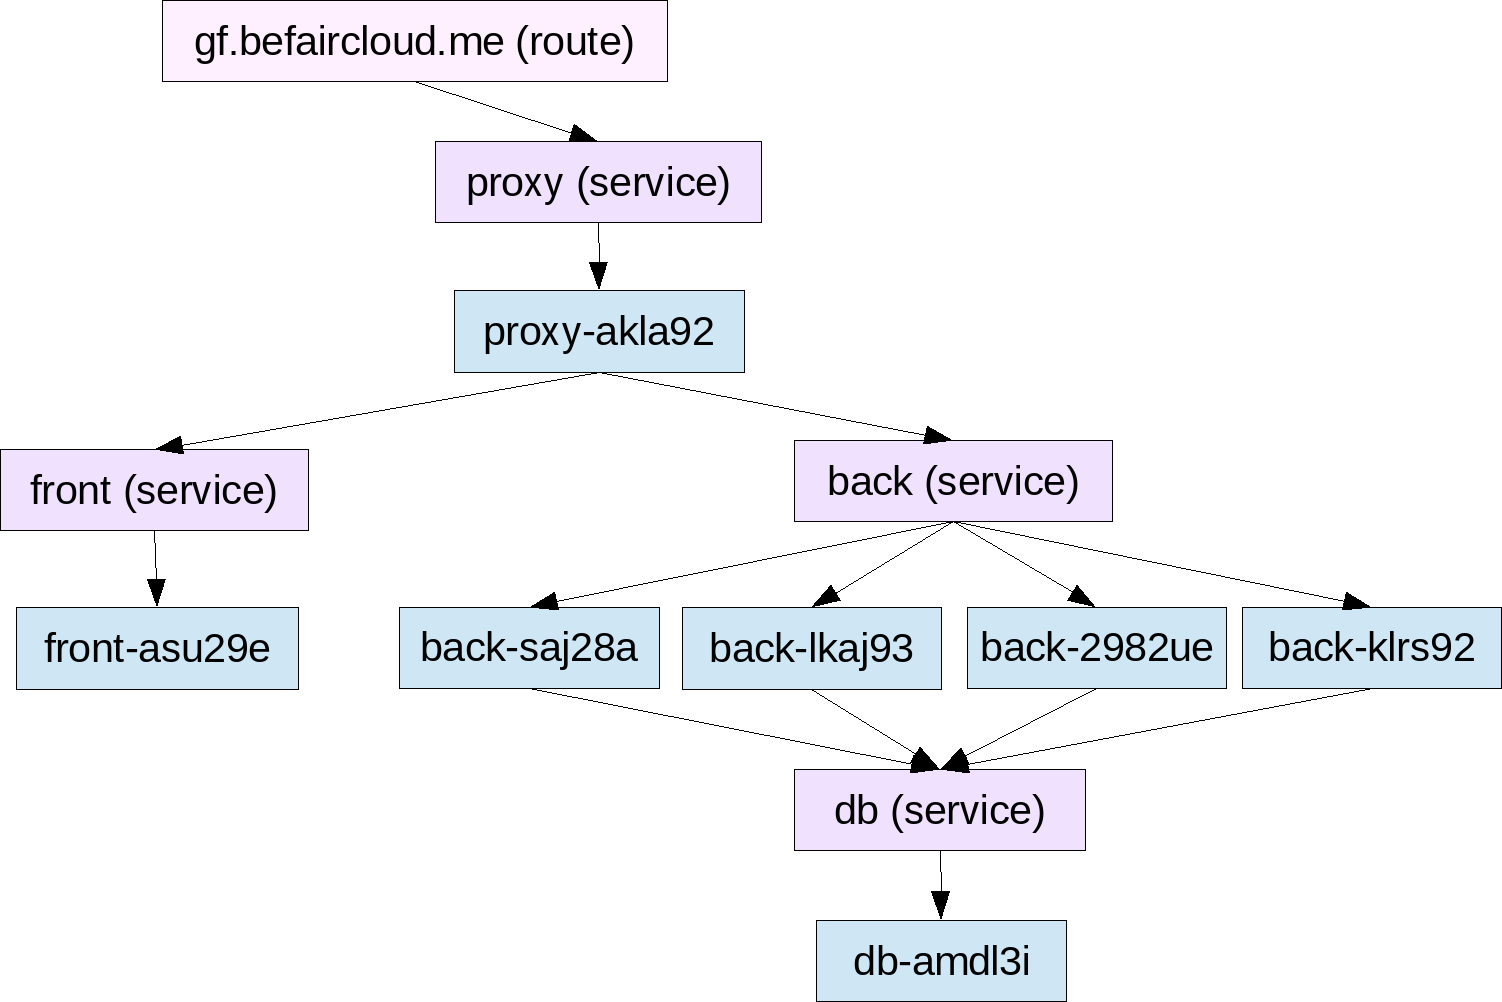
\includegraphics{media/ch5-template-gf.png}
\caption{Gasista Felice template}
\end{figure}

In details:

\begin{itemize}
\itemsep1pt\parskip0pt\parsep0pt
\item
  \emph{database}: while in development the default
  \texttt{postgresql:9.4} image worked fine, on OpenShift it had some
  problems probably due to permissions. So it has been used a dedicated
  image for OpenShift, providing PostgreSQL 9.2, also compatible with
  Gasista Felice. As of other RDBMS, PostgreSQL by design is composed by
  a unique master, and for major scalability in reads, could be setted
  up some slaves but it's not needed.
\item
  The \emph{backend} is the component of uWSGI, Python and Django is the
  main one on which it's possible act. At the end of chapter will be
  provided some benchmarks.
\item
  The \emph{frontend} is mainly useful in development, but in production
  once it has generated the files, it could be cached from NGiNX. In
  further optimization, this component will be deleted at all, and the
  static files will be served directly. In this case will be use
  \texttt{1} replica since there is no need of scaling this component.
\item
  \emph{Proxy} component, NGiNX represent the entry point of the
  application, so it manages caching of static content, demanding to the
  \texttt{front} and \texttt{back} non-cached requests. Since NGiNX is
  generally enough fast thanks to asynchronous loops, should not be
  necessary adding further pods.
\end{itemize}

\section{Benchmarks}\label{benchmarks}

One of the goal of this project is analyze the component for
scalability. Kubernetes's provide the horizontal scaling of pods, so has
been done some benchmarks varying the number of pods of Gasista Felice
backend.

The test consists in using \emph{boom} for 100 concurrent requests for a
total of 100 requests, that consist in a \emph{GET} at
\texttt{/gasistafelice} path of the application, so a
\texttt{GET\ http://gf.befaircloud.me/gasistafelice} in this case. Even
if this should be a simple request, instead involves several work and
represent a simple but significant test case. The values registered
consist in:

\begin{itemize}
\itemsep1pt\parskip0pt\parsep0pt
\item
  \emph{total time}: interval from the beginning of the first request,
  to the end of the last requests
\item
  \emph{requests per second}: represent the medium of requests served
  per second
\end{itemize}

\begin{longtable}[c]{@{}lll@{}}
\caption{Benchmark results}\tabularnewline
\toprule
Backend pods & total time & reqs/s\tabularnewline
\midrule
\endfirsthead
\toprule
Backend pods & total time & reqs/s\tabularnewline
\midrule
\endhead
1 & 34s & 2.5reqs/s\tabularnewline
2 & 33s & 2.7reqs/s\tabularnewline
3 & 26s & 3.7reqs/s\tabularnewline
4 & 20s & 4.8reqs/s\tabularnewline
8 & 22s & 4.5reqs/s\tabularnewline
\bottomrule
\end{longtable}

The results the decreasing time with adding additional pods, to 4 pods.
Beyond 4 pods there is no advantage, probably because of cluster
resource limit.
\chapter{Monitoring and Logging}\label{monitoring-and-logging}

This chapter shows how to control, monitor, analyze, and visualize
metrics about applications, doing some benchmark to test che scalability
of the apps on this stack.

Monitoring the system resources and logging of applications should be a
first-class task in IT Operations, because it's not possible control
what it's not possible measure. Traditional tools are generally hard to
configure and it needs to create a dedicated transport layer (with
encryption/authentication) of various components between hosts. Luckily,
in this situation it's possible take advantage of the cluster primitives
to make it an easier (and efficient) task.

While \emph{InfluxDB} and \emph{Grafana} are a popular choice
respectively for storage and visualize resource metrics, in logging
world the most popular one is the \emph{ELK} stack, where ELK stands for
\emph{ElasticSearch} (storage), \emph{Logstash} (log processing) and
\emph{Kibana} (visualization). Since a guideline is the lightweight,
instead of using an additional stack for logging, it has been reused
both InfluxDB and Grafana, adding \emph{Heka} for logs processing, so
the stack could be called \emph{IHG}: InfluxDB, Heka and Grafana.

In addition, Kubernetes' kubelet comes with built-in \emph{cAdvisor} for
resource monitoring, while \emph{Heapster} is the main plug-in for
resource cluster manager. At the end, Logspout (built-in in recent
versions of Heka) will be used for gathering logs from all running
containers.

\begin{figure}[htbp]
\centering
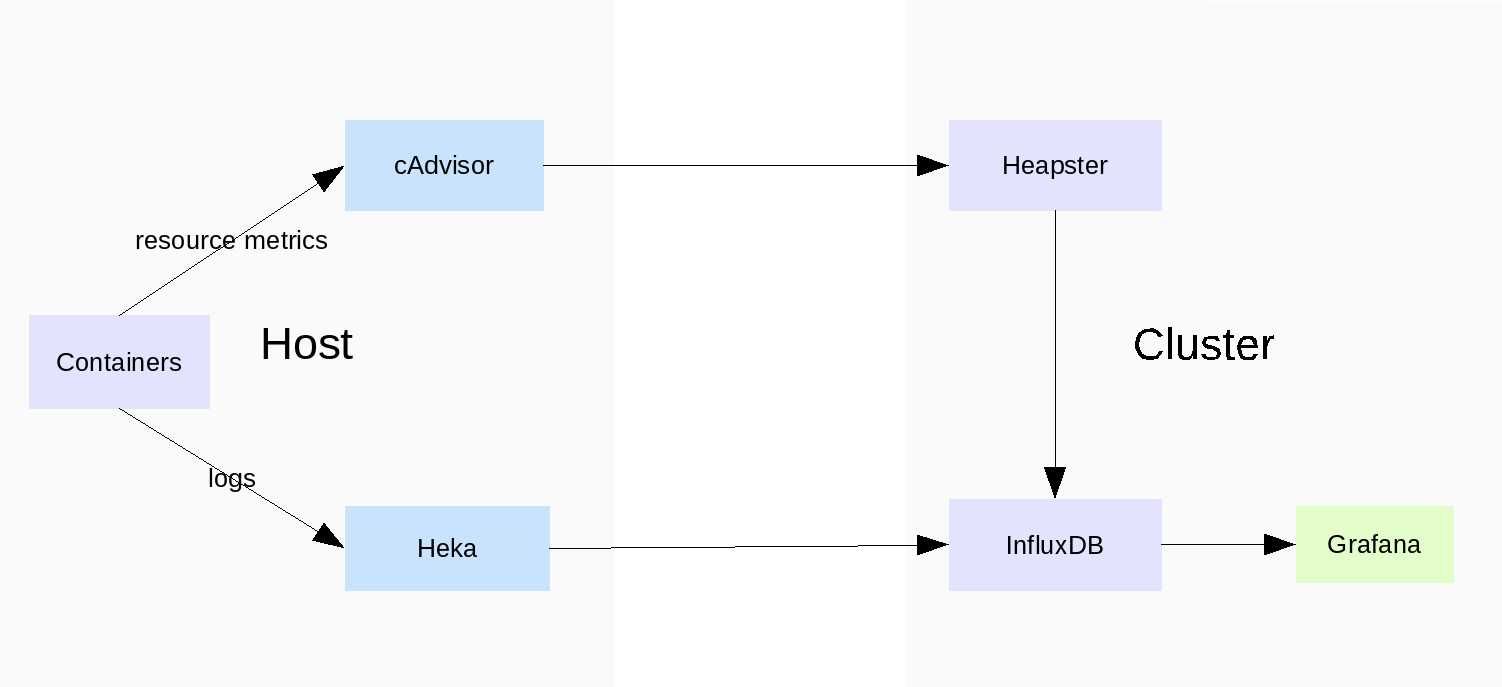
\includegraphics{media/ch6-overview.png}
\caption{Overview of monitoring system}
\end{figure}

The monitoring stack is deployed as an unique application, and includes
\texttt{ReplicationController}s, \texttt{Service}s but also
\texttt{Route}s for external reachability:

\section{Time-Series Storage}\label{time-series-storage}

InfluxDB is a distributed time-series database that fits well since it
doesn't need a pre-defined schema for data, it's horizontally scalable
in the NoSQL way, support native data replication and include a familiar
SQL-like language, \emph{InfluxQL}.

InfluxQL is the query language. Here some examples:

\begin{verbatim}
select * from mem_usage

select * from log_lines where line =~ /error/i

select mean(cpu_load) group by time(30m) where time > now() - 1d and host = 'server E'
\end{verbatim}

Resource:

\begin{verbatim}
[{
  "name": "load_avg",
  "columns": [
    "time",
    "app",
    "value"
  ],
  "points": [[
    1400425342091,
    "Frontend B",
    0.8
  ]]
}]
\end{verbatim}

Log:

\begin{verbatim}
[{
  "name": "log_lines",
  "columns": [
    "time",
    "app",
    "line"
  ],
  "points": [[
    1400425947368,
    "Frontend B",
    "some useful log info"
  ]]
}]
\end{verbatim}

In OpenShift, InfluxDB runs as component of monitoring application, and
is composed by a \texttt{replicationController} and a \texttt{service}:

\section{Resource Gathering}\label{resource-gathering}

Kubernetes comes with built-in cAdvisor
(https://github.com/google/cadvisor) in Kubelet, for resource metrics
gathering, such as CPU, RAM, I/O, network, etc.

Heapster (https://github.com/kubernetes/heapster) is the Kubernetes
cluster monitoring system, that gather metrics from nodes and send them
to InfluxDB.

The exported metrics are:

\begin{itemize}
\itemsep1pt\parskip0pt\parsep0pt
\item
  uptime: Number of milliseconds since the container was started
\item
  cpu/usage: Cumulative CPU usage on all cores
\item
  cpu/limit: CPU limit in millicores
\item
  memory/usage: Total memory usage
\item
  memory/working\_set: Total working set usage. Working set is the
  memory being used and not easily dropped by the kernel
\item
  memory/limit: Memory limit
\item
  memory/page\_faults: Number of page faults
\item
  memory/major\_page\_faults: Number of major page faults
\item
  network/rx: Cumulative number of bytes received over the network
\item
  network/rx\_errors: Cumulative number of errors while receiving over
  the network
\item
  network/tx: Cumulative number of bytes sent over the network
\item
  network/tx\_errors: Cumulative number of errors while sending over the
  network
\item
  filesystem/usage: Total number of bytes consumed on a filesystem
\item
  filesystem/limit: The total size of filesystem in bytes
\end{itemize}

While the exported labels are:

\begin{itemize}
\itemsep1pt\parskip0pt\parsep0pt
\item
  hostname: Hostname where the container ran
\item
  host\_id: Identifier specific to a host. Set by cloud provider or user
\item
  container\_name: User-provided name of the container or full container
  name for system containers
\item
  pod\_name: The name of the pod
\item
  pod\_id: The unique ID of the pod
\item
  pod\_namespace: The namespace of the pod
\item
  namespace\_id: The UID of namespace of the pod
\item
  labels: Comma-separated list of user-provided labels
\item
  resource\_id: Identifier(s) specific to a metric
\end{itemize}

Heapster is deployed as \texttt{replicationController}, a
\texttt{service} and a \texttt{route}.

\section{Log Processing}\label{log-processing}

\emph{Heka} is a framework developed by Mozilla for easy data collection
and processing. Heka is modular and supports mainly 6 different type of
plugins: inputs, splitters, decoders, filters, encoders and outputs. The
first 3 are for gather and parse incoming data to \emph{Heka Message}
standard, the filters parse all theese messages and the later 2 is for
encoding and sending data somewhere else, for storaging or further
processing.

Heka permits to logs parsing, filtering, structuring them and send to
InfluxDB. In this example will use Gasista Felice's NGiNX component for
generating logs and \emph{boom} for doing a lot of requests.

\begin{figure}[htbp]
\centering
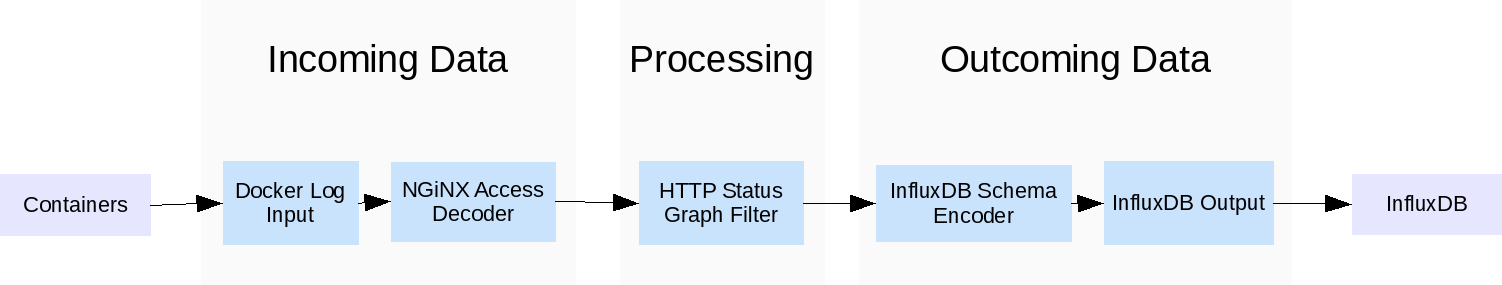
\includegraphics{media/ch6-heka.png}
\caption{The Heka Data Flow}
\end{figure}

The input part is composed by the \emph{Docker Log Input}, build on top
of \emph{Logspout} that acquires stdout/stderr of running containers
from the Docker Engine Unix socket, and \emph{NGiNX access} and
\emph{error decoders}.

Filtering consist of \emph{HTTP Status Graph} that filter NGiNX access
logs and generate an HTTP response code based graph.

The output part is composed by encoding in \emph{InfluxDB schema} and
sending data to \emph{InfluxDB HTTP APIs}.

Heka is deployed on top of OpenShift as a simple
\texttt{ReplicationController}.

\section{Data Visualization}\label{data-visualization}

Grafana is a metrics dashboard and graph editor, born as fork of Kibana
in the beginning of 2014.

\begin{figure}[htbp]
\centering
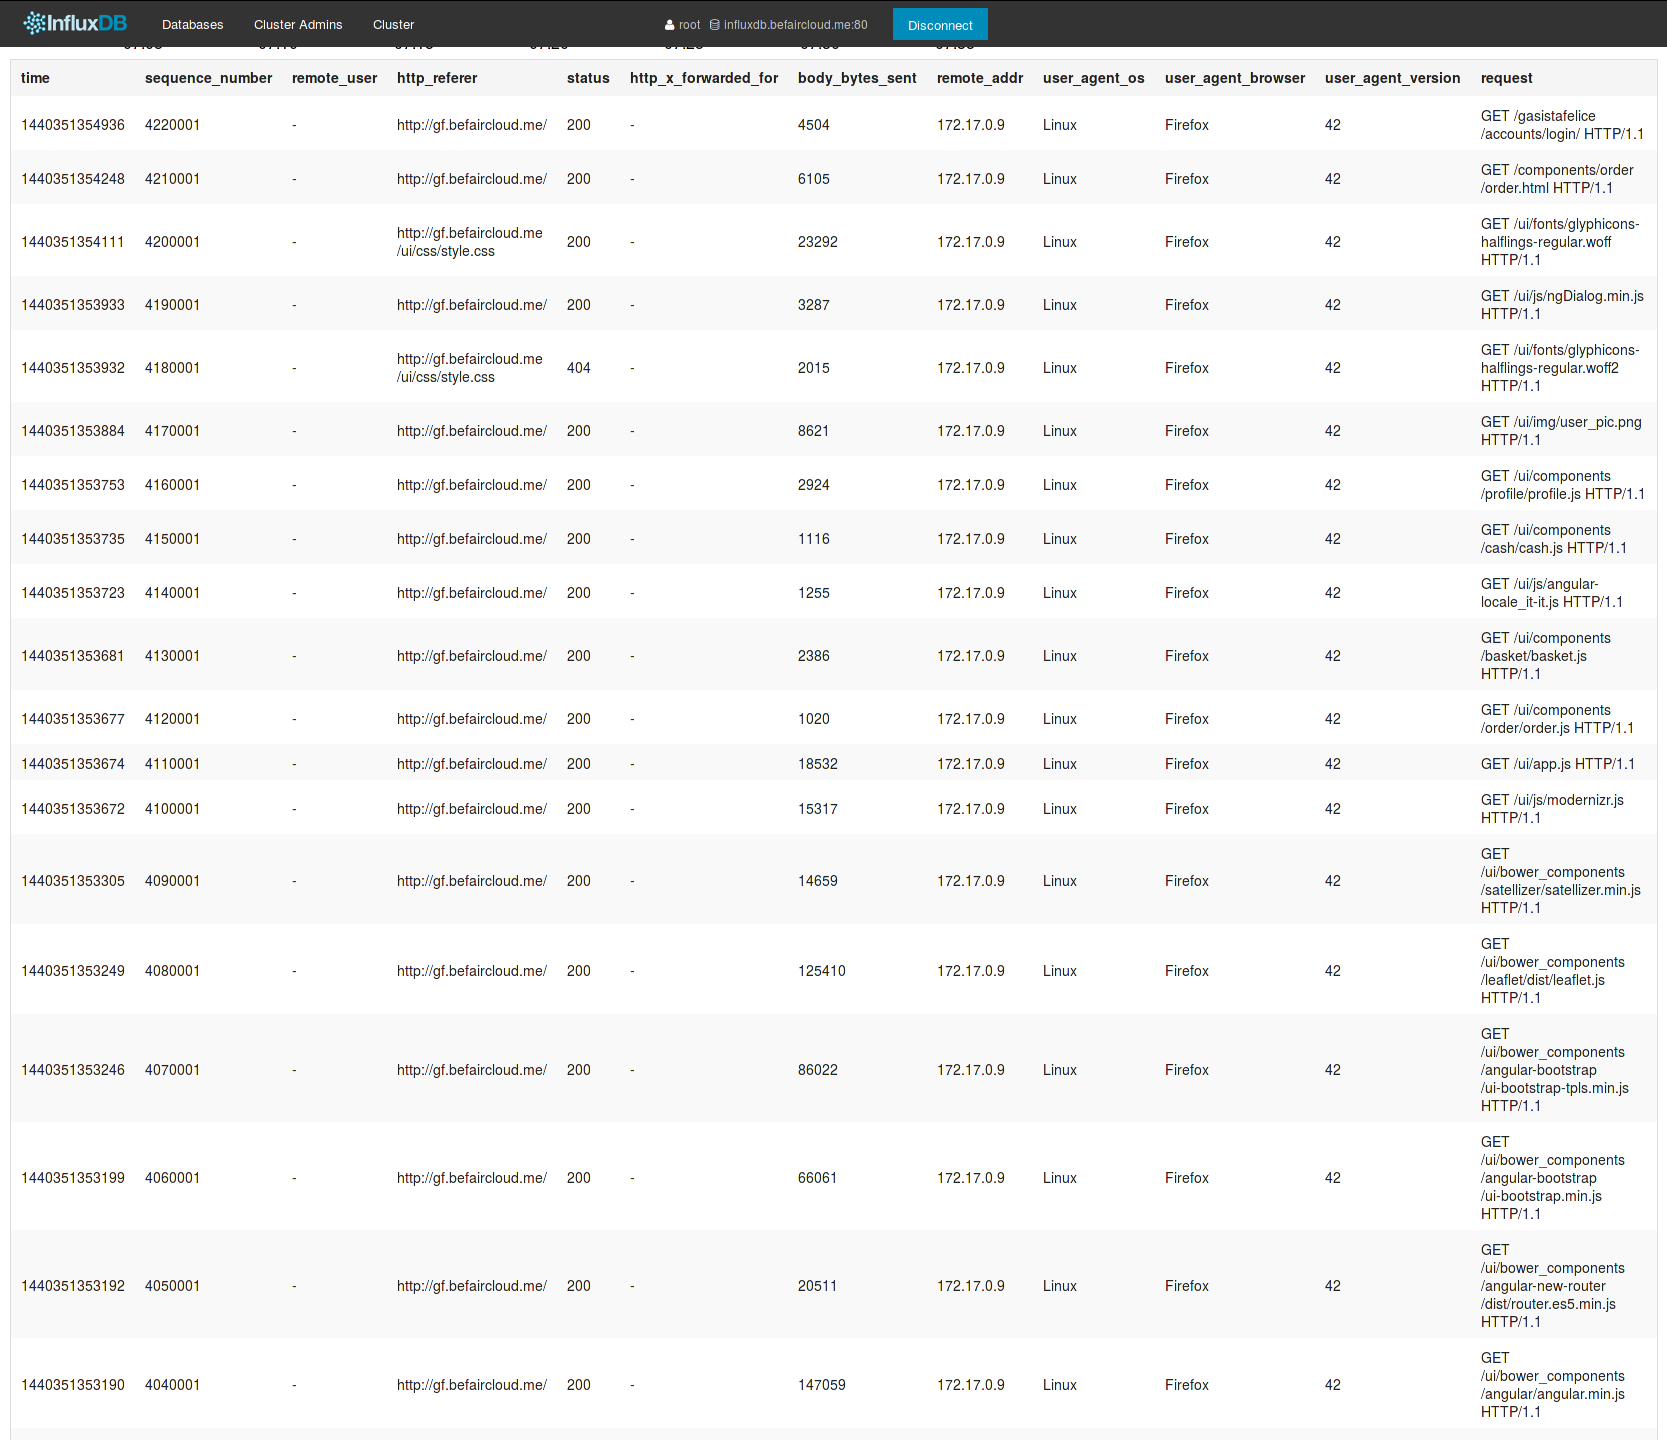
\includegraphics{media/ch6-influxdb.png}
\caption{InfluxDB logs dashboard}
\end{figure}

\begin{figure}[htbp]
\centering
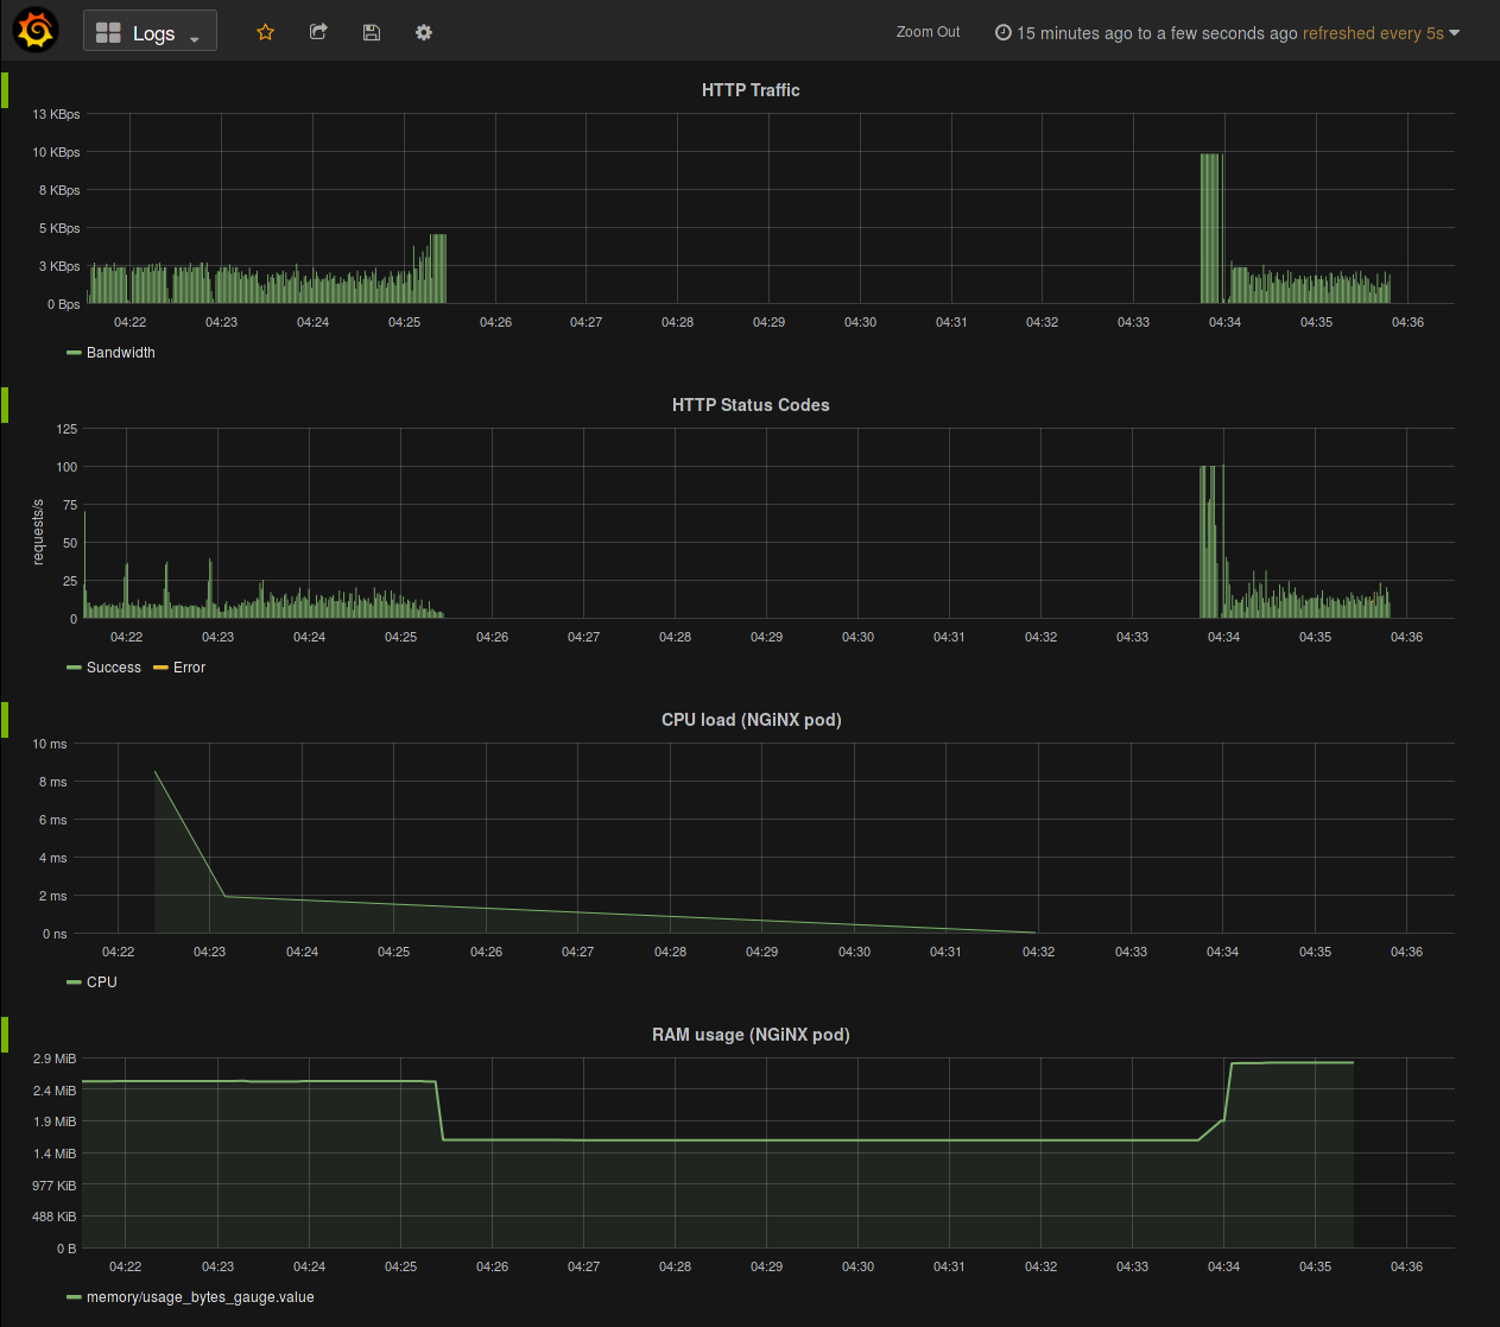
\includegraphics{media/ch6-grafana.png}
\caption{Grafana logs dashboard}
\end{figure}

Grafana is deployed with a \texttt{ReplicationController}, a
\texttt{Service} and a \texttt{Route} in order to be reached from the
external.

\section{Benchmarks}\label{benchmarks}

One of the goal of this project is analyze the component for
scalability. Kubernetes's provide the horizontal scaling of pods, so has
been done some benchmarks varying the number of pods of Gasista Felice
backend.

The test consists in using \emph{boom} for 100 concurrent requests for a
total of 100 requests, that consist in a \emph{GET} at
\texttt{/gasistafelice} path of the application, so a
\texttt{GET\ http://gf.befaircloud.me/gasistafelice} in this case. Even
if this should be a simple request, instead involves several work and
represent a simple but significant test case. The values registered
consist in:

\begin{itemize}
\itemsep1pt\parskip0pt\parsep0pt
\item
  \emph{total time}: interval from the beginning of the first request,
  to the end of the last requests
\item
  \emph{requests per second}: represent the medium of requests served
  per second
\end{itemize}

\begin{longtable}[c]{@{}lll@{}}
\caption{Benchmark results}\tabularnewline
\toprule
Backend pods & total time & reqs/s\tabularnewline
\midrule
\endfirsthead
\toprule
Backend pods & total time & reqs/s\tabularnewline
\midrule
\endhead
1 & 34s & 2.5reqs/s\tabularnewline
2 & 33s & 2.7reqs/s\tabularnewline
3 & 26s & 3.7reqs/s\tabularnewline
4 & 20s & 4.8reqs/s\tabularnewline
8 & 22s & 4.5reqs/s\tabularnewline
\bottomrule
\end{longtable}

The results the decreasing time with adding additional pods, to 4 pods.
Beyond 4 pods there is no advantage, probably because of cluster
resource limit.
\chapter{Conclusions}\label{conclusions}

\section{Summary}\label{summary}

Containers and emerging ecosystem around them are questioning the whole
IT industry about the role of the OS today. There are several new
opportunity for radically enhance the development and operations
workflow, software architecture and application environments.

Docker is a new and pretty immature runtime, but the promises around it
there are. Kubernetes on the other side, as scheduling and orchestration
framework, has been adopted from other PaaS beyond OpenShift, like Deis,
and from lower-level components, like Mesos.

\section{Future Developments}\label{future-developments}

At this point, there are a large variety of potential improvements.

From the monitoring and logging point of view, could be enabled an
alerting system directly via Heka alert encoder plug-in, or via a
dedicated software like \emph{Sentry} or \emph{Bosun}.

The main point is \emph{high availability}\cite{HighAvailability}.

Applications running on top of the platform that use traditional
relational database such as PostgreSQL, could be configured for high
availability also for data
(https://www.compose.io/articles/high-availability-for-postgresql-batteries-not-included/).

From the cluster perspective, there is the possibility of rolling update
or auto-scaling of the cluster itself. In fact with passing the time,
the stack should be updated, and the applications deployed on cluster
could need globally more resources. A way to do this is monitoring the
global load of the cluster, and instruct Terraform for vary the number
of nodes accordingly to it.

Beyond the single cluster, there is an emerging proposal for
\emph{cluster federation}, called Ubernetes, that enables
high-availability with geographically distributed Kubernetes clusters.

With that global distributed infrastructure, it's possible build
geographycally distributed applications built on top of databases like
Consul for key-value storage or CockroachDB for more complex cases.

\appendix
\chapter{Source code}\label{source-code}

\section{Gasista Felice}\label{gasista-felice}

\subsection{Dockerfile of NGiNX base
image}\label{dockerfile-of-nginx-base-image}

\begin{verbatim}
FROM nginx:1.9

MAINTAINER Antonio Esposito "kobe@befair.it"

RUN rm -rf /etc/nginx/conf.d/*
COPY nginx.conf /etc/nginx/nginx.conf
\end{verbatim}

\subsection{NGiNX base configuration
file}\label{nginx-base-configuration-file}

\begin{verbatim}
user  nginx;
worker_processes  1;
error_log  stderr warn;
pid        /var/run/nginx.pid;


events {
    worker_connections  1024;
}


http {
    include       /etc/nginx/mime.types;
    default_type  application/octet-stream;

    log_format  main  '$remote_addr - $remote_user [$msec] "$request" '
                      '$status $body_bytes_sent "$http_referer" '
                      '"$http_user_agent" "$http_x_forwarded_for"';

    access_log  /dev/stdout  main;

    sendfile        on;
    #tcp_nopush     on;

    keepalive_timeout  65;

    #gzip  on;

    server_tokens            off;
    server_name_in_redirect  off;
    port_in_redirect         off;

    include /etc/nginx/conf.d/*.conf;
}
\end{verbatim}

\subsection{Proxy's Dockerfile}\label{proxys-dockerfile}

\begin{verbatim}
FROM kobe25/nginx:latest

MAINTAINER Antonio Esposito "kobe@befair.it"

COPY site.conf /etc/nginx/conf.d/site.conf
\end{verbatim}

\subsection{NGiNX configuration file}\label{nginx-configuration-file}

\begin{verbatim}
server {
  listen 8080 default_server;

  server_name _;
  root /code;

  charset utf-8;
  client_max_body_size 75M;
  client_body_timeout 600s;

  location = /favicon.ico {
    log_not_found off;
    access_log off;
  }

  location = /robots.txt {
    allow all;
    log_not_found off;
    access_log off;
  }

  location ~ /\. {
    deny all;
    log_not_found off;
    access_log off;
  }

  location = / {
    proxy_pass      http://front:5000/ui/index.html;
    expires max;
  }

  location /components/ {
    proxy_pass      http://front:5000/ui/components/;
    expires max;
  }

  location /ui/bower_components/ {
    proxy_pass      http://front:5000/libs/bower_components/;
    expires max;
  }

  location /ui/ {
    proxy_pass      http://front:5000;
    expires max;
  }

  location /static/ {
    include          uwsgi_params;
    uwsgi_pass       uwsgi://back:5000;
    expires max;
  }

  location /media/ {
    include          uwsgi_params;
    uwsgi_pass       uwsgi://back:5000;
  }

  location /api/ {
    gzip             on;
    gzip_types       application/json;
    gzip_min_length  1000;

    include          uwsgi_params;
    uwsgi_pass       uwsgi://back:5000;
  }

  location /gasistafelice/ {
    include          uwsgi_params;
    uwsgi_pass       uwsgi://back:5000;
  }

  location / {
    return 404;
  }
}
\end{verbatim}

\subsection{Dockerfile of uWSGI/Python2 base
image}\label{dockerfile-of-uwsgipython2-base-image}

\begin{verbatim}
FROM python:2.7.7

MAINTAINER Antonio Esposito "kobe@befair.it"

ENV DEBIAN_FRONTEND         noninteractive

ENV PYTHONUNBUFFERED        1
ENV PYTHONPATH              /code:/usr/local/lib/python2.7/site-packages
ENV UWSGI_CALLABLE          app

ENV UWSGI_MASTER            true
ENV UWSGI_MASTER_AS_ROOT    true
ENV UWSGI_UID               app
ENV UWSGI_GID               app
ENV UWSGI_UWSGI_SOCKET      0.0.0.0:5000
ENV UWSGI_NO_ORPHANS        true
ENV UWSGI_VACUUM            true
ENV UWSGI_LOG_DATE          true

ENV UWSGI_WORKERS           4
ENV UWSGI_THREADS           1
ENV UWSGI_ENABLE_THREADS    true
ENV UWSGI_BUFFER_SIZE       65536
ENV UWSGI_MAX_REQUESTS      128
ENV UWSGI_HARAKIRI          120
ENV UWSGI_HARAKIRI_VERBOSE  true
ENV UWSGI_THUNDER_LOCK      true

ENV PGDATABASE              app
ENV PGUSER                  app
ENV PGPASSWORD              app
ENV PGHOST                  db
ENV PGPORT                  5432

RUN groupadd -r app && \
    useradd -r -g app -d /code app

RUN apt update && \
    apt install -y \
      build-essential \
      python-dev \
      python-setuptools && \
    rm -rf /var/lib/apt/lists/*
RUN pip install \
      'uWSGI >=2.0, <2.1'

EXPOSE 5000
CMD ["uwsgi"]
\end{verbatim}

\subsection{Backend's Dockerfile}\label{backends-dockerfile}

\begin{verbatim}
FROM kobe25/uwsgi-python2:latest

MAINTAINER Antonio Esposito "kobe@befair.it"

ENV LC_ALL                  it_IT.UTF-8
ENV LANG                    it_IT.UTF-8
ENV LANGUAGE                it_IT.UTF-8

ENV PYTHONPATH
    /code:/code/gasistafelice:/usr/local/lib/python2.7/site-packages
ENV UWSGI_CHDIR             /code/gasistafelice
ENV UWSGI_WSGI_FILE         /code/gasistafelice/gf/wsgi.py
ENV DJANGO_SETTINGS_MODULE  gf.settings
ENV UWSGI_STATIC_MAP        /static=/code/gasistafelice/static
ENV UWSGI_STATIC_SAFE
    /usr/local/lib/python2.7/site-packages/django/contrib/admin/static/admin

COPY deps/debian /code/gasistafelice/deps/debian
RUN apt update && \
    apt install -y $(cat /code/gasistafelice/deps/debian) && \
    rm -rf /var/lib/apt/lists/*

COPY deps/locale.gen /etc/locale.gen
RUN locale-gen

COPY deps/ /code/gasistafelice/deps/
RUN pip install -r /code/gasistafelice/deps/dev.txt

COPY ./ /code/gasistafelice/
WORKDIR /code/gasistafelice/
\end{verbatim}

\subsection{Frontend's Dockerfile}\label{frontends-dockerfile}

\begin{verbatim}
FROM iojs:2.5

MAINTAINER Antonio Esposito "kobe@befair.it"

COPY deps/npm /code/ui/deps/npm
RUN npm install -g $(cat /code/ui/deps/npm)

COPY ./bower.json /code/libs/bower.json
RUN cd /code/libs/ && bower install --allow-root

EXPOSE 5000

COPY ./ /code/ui/
WORKDIR /code/ui/

CMD ["harp", "server", "-i", "0.0.0.0", "-p", "5000", "/code"]
\end{verbatim}

\subsection{Docker Compose file}\label{docker-compose-file}

\begin{verbatim}
proxy:
  image: befair/gasistafelice-proxy:latest
  volumes:
    - ./proxy/site.conf.dev:/etc/nginx/conf.d/site.conf:ro
  ports:
    - '127.0.0.1:8080:8080'
  links:
    - front
    - back

front:
  image: befair/gasistafelice-front:latest
  volumes:
    - ./ui:/code/ui:rw

back:
  image: befair/gasistafelice-back:latest
  volumes:
    - ./gasistafelice:/code/gasistafelice:ro
    - ./gasistafelice/fixtures:/code/gasistafelice/fixtures:rw
    - /tmp/gf_tracebacker:/tmp/tracebacker:rw
    - /tmp/gf_profiling:/tmp/profiling:rw
  ports:
    - '127.0.0.1:7000:7000'
  links:
    - db
  env_file: ./compose/settings.env

db:
  image: postgres:9.4
  env_file: ./compose/settings.env
\end{verbatim}

\subsection{OpenShift template}\label{openshift-template}

\begin{verbatim}
apiVersion: v1
kind: Template
metadata:
  name: gasistafelice
  annotations:
    description: >
      Gasista Felice is the platform for DES Macerata project
    tags: app,gas,des
labels:
  app: gf
  application: gasistafelice
parameters:
-
  name: ENV
  description: dev/stage/prod environment
  value: prod
-
  name: SERVER_NAME
  description: server name
-
  name: POSTGRES_PASSWORD
  description: Password used for DB authentication
  generate: expression
  from: '[\w]{12}'
objects:
-
  apiVersion: v1
  kind: ReplicationController
  metadata:
    name: db
    labels:
      name: db
  spec:
    replicas: 1
    selector:
      name: db
    template:
      metadata:
        labels:
          name: db
      spec:
        volumes:
        -
          name: postgres-ps
          emptyDir: {}
        containers:
        -
          name: db
          image: openshift/postgresql-92-centos7
          env:
          -
            name: POSTGRESQL_USER
            value: app
          -
            name: POSTGRESQL_PASSWORD
            value: ${POSTGRES_PASSWORD}
          -
            name: POSTGRESQL_DATABASE
            value: app
          -
            name: POSTGRESQL_ADMIN_PASSWORD
            value: ${POSTGRES_PASSWORD}
          ports:
          -
            name: postgresql-port
            containerPort: 5432
          volumeMounts:
          -
            name: postgres-ps
            mountPath: /var/lib/pgsql/data
            readOnly: false
-
  apiVersion: v1
  kind: Service
  metadata:
    name: db
    labels:
      name: db
  spec:
    ports:
    -
      port: 5432
      targetPort: postgresql-port
    selector:
      name: db
-
  apiVersion: v1
  kind: ReplicationController
  metadata:
    name: back
  spec:
    replicas: 1
    selector:
      name: back
    template:
      metadata:
        labels:
          name: back
      spec:
        containers:
        -
          name: back
          image: befair/gasistafelice-back
          ports:
          -
            name: back-port
            containerPort: 5000
          env:
          -
            name: APP_ENV
            value: ${ENV}
          -
            name: APP_SERVER_NAME
            value: ${SERVER_NAME}
          -
            name: POSTGRES_USER
            value: app
          -
            name: POSTGRES_PASSWORD
            value: ${POSTGRES_PASSWORD}
          -
            name: POSTGRESQL_USER
            value: app
          -
            name: POSTGRESQL_PASSWORD
            value: ${POSTGRES_PASSWORD}
          -
            name: POSTGRESQL_DATABASE
            value: app
          -
            name: POSTGRESQL_ADMIN_PASSWORD
            value: ${POSTGRES_PASSWORD}
          -
            name: PGUSER
            value: app
          -
            name: PGPASSWORD
            value: ${POSTGRES_PASSWORD}
-
  apiVersion: v1
  kind: Service
  metadata:
    name: back
  spec:
    ports:
    -
      port: 5000
      targetPort: back-port
    selector:
      name: back
-
  apiVersion: v1
  kind: ReplicationController
  metadata:
    name: front
  spec:
    replicas: 1
    selector:
      name: front
    template:
      metadata:
        labels:
          name: front
      spec:
        containers:
        -
          name: front
          image: befair/gasistafelice-front
          ports:
          -
            name: front-port
            containerPort: 5000
-
  apiVersion: v1
  kind: Service
  metadata:
    name: front
  spec:
    ports:
    -
      port: 5000
      targetPort: front-port
    selector:
      name: front
-
  apiVersion: v1
  kind: ReplicationController
  metadata:
    name: proxy
  spec:
    replicas: 1
    selector:
      name: nginx
    template:
      metadata:
        labels:
          name: nginx
      spec:
        volumes:
        -
          name: nginx-cache
          emptyDir: {}
        -
          name: nginx-run
          emptyDir: {}
        containers:
        -
          name: proxy
          image: befair/gasistafelice-proxy
          securityContext:
            runAsUser: 0
            privileged: true
          ports:
          -
            name: insecure-port
            containerPort: 8080
          volumeMounts:
          -
            name: nginx-cache
            mountPath: /var/cache/nginx
            readOnly: false
          -
            name: nginx-run
            mountPath: /var/run
            readOnly: false
-
  apiVersion: v1
  kind: Service
  metadata:
    name: proxy
  spec:
    selector:
      name: nginx
    ports:
    -
      port: 8080
      targetPort: insecure-port
-
  apiVersion: v1
  kind: Route
  metadata:
    name: route
  spec:
    host: ${SERVER_NAME}
    to:
      kind: Service
      name: proxy
\end{verbatim}

\section{IaaS and PaaS bootstrapping}

\subsection{Makefile}\label{makefile}

\begin{verbatim}
NETENV_V := 1.0.0
TF_V := 0.6.3
OS_V := 1.0.5
OS_COMMIT := 96963b6

BINPATH := ${GOPATH}/bin
export PATH := ${GOPATH}/bin:${PATH}
TF_URL := https://dl.bintray.com/mitchellh/terraform/\
    terraform_${TF_V}_linux_amd64.zip
OS_URL := https://github.com/openshift/origin/releases/download/\
    v${OS_V}/openshift-origin-v${OS_V}-${OS_COMMIT}-linux-amd64.tar.gz
NETENV_URL := https://github.com/kelseyhightower/\
    setup-network-environment/releases/download/\
    v${NETENV_V}/setup-network-environment


help:
        @cat Makefile

install:
        @mkdir -p .cache
        @go get -u github.com/dbohdan/remarshal
        @go get -u github.com/rakyll/boom
        @go install github.com/dbohdan/remarshal
        @go install github.com/rakyll/boom
        @curl -L -o .cache/setup-network-environment \
            -z .cache/setup-network-environment ${NETENV_URL}
        @curl -L -o .cache/terraform.zip \
            -z .cache/terraform.zip             ${TF_URL}
        @curl -L -o .cache/openshift-origin.tar.gz \
            -z .cache/openshift-origin.tar.gz   ${OS_URL}
        @unzip -o   .cache/terraform.zip             -d ${BINPATH}/
        @tar -xf    .cache/openshift-origin.tar.gz   -C .cache/
        @ln -sf     .cache/openshift ${BINPATH}/openshift
        @ln -sf     ${BINPATH}/openshift ${BINPATH}/oc
        @ln -sf     ${BINPATH}/openshift ${BINPATH}/oadm

clean soft-clean:
        @rm -rf \
                terraform.* \
                .cache/*.{gz,zip,toml} \
                .cache/master/ \
                .cache/id*

full-clean: clean
        @rm -rf \
                ${BINPATH}/terraform* \
                .cache/

compile:
        @mkdir -p .cache
        @remarshal \
                -if yaml -i terraform/digitalocean.yaml \
                -of json -o terraform.tf.json
        @remarshal \
                -if yaml -i vars.yaml \
                -of json -o terraform.tfvars

up: clean compile
        @ssh-keygen -b 4096 -t rsa -f .cache/id -N ''
        @tar -czf .cache/pkg.tar.gz \
                openshift/ \
                .cache/{setup-network-environment,openshift}
        @terraform plan -out terraform.tfplan
        @terraform apply terraform.tfplan

delete destroy: compile
        @terraform plan -destroy
        @terraform destroy

infrastructure-graph:
        @terraform graph | dot -Tsvg > graph.svg

test:
        @./benchmark
\end{verbatim}

\subsection{Terraform template for Digital
Ocean}\label{terraform-template-for-digital-ocean}

\begin{verbatim}
variable:
  BASE_DOMAIN: { default: befaircloud.me }
  NODES: { default: 2 }
  OMASTER: { default: /opt/bin/openshift.local.config/master }
  ONODE: { default: /opt/bin/openshift.local.config/node }
  # Provider specific
  DO_TOKEN:       {}
  DO_SSH_ID:      { default: core }
  DO_IMAGE:       { default: coreos-beta }
  DO_REGION:      { default: fra1 }
  DO_MASTER_SIZE: { default: 1gb }
  DO_NODE_SIZE:   { default: 2gb }

provider:
  digitalocean:
    token: ${var.DO_TOKEN}

resource:
  template_file:
    master_conf:
      filename: terraform/master.yaml
      vars:
        HOME: /home/core
        OMASTER: ${var.OMASTER}
        SSH_PUBLIC_KEY: ${file(".cache/id.pub")}
        BASE_DOMAIN: ${var.BASE_DOMAIN}
        NODES: ${var.NODES}

    node_conf:
      filename: terraform/node.yaml
      vars:
        HOME: /home/core
        OMASTER: ${var.OMASTER}
        ONODE: ${var.ONODE}
        MASTER_IP: >
          ${digitalocean_droplet.master.ipv4_address_private}
        SSH_PUBLIC_KEY: ${file(".cache/id.pub")}
      depends_on:
      - digitalocean_droplet.master

  digitalocean_ssh_key:
    superuser:
      name: ${var.DO_SSH_ID}
      public_key: ${file(".cache/id.pub")}
  digitalocean_droplet:
    master:
      image: ${var.DO_IMAGE}
      name: master
      region: ${var.DO_REGION}
      size: ${var.DO_MASTER_SIZE}
      ipv6: true
      private_networking: true
      user_data: ${template_file.master_conf.rendered}
      ssh_keys:
      - ${digitalocean_ssh_key.superuser.fingerprint}
      depends_on:
      - template_file.master_conf
      connection:
        user: core
        key_file: .cache/id
      provisioner:
        file:
          source: .cache/pkg.tar.gz
          destination: /home/core/pkg.tar.gz
        remote-exec:
          inline:
          - sudo mkdir -p /opt/bin/
          - tar -xf /home/core/pkg.tar.gz -C /home/core
          - sudo mv /home/core/.cache/setup-network-environment \
              /opt/bin/
          - sudo mv /home/core/.cache/openshift /opt/bin/
          - mv /home/core/openshift/* /home/core/
          - rm -rf /home/core/{pkg.tar.gz,.cache,openshift}

    nodes:
      count: ${var.NODES}
      image: ${var.DO_IMAGE}
      name:  node-${count.index}
      region: ${var.DO_REGION}
      size: ${var.DO_NODE_SIZE}
      ipv6: true
      private_networking: true
      user_data: ${template_file.node_conf.rendered}
      ssh_keys:
      - ${digitalocean_ssh_key.superuser.fingerprint}
      depends_on:
      - digitalocean_droplet.master
      - template_file.node_conf
      connection:
        user: core
        key_file: .cache/id
      provisioner:
        file:
          source: .cache/pkg.tar.gz
          destination: /home/core/pkg.tar.gz
        remote-exec:
          inline:
          - sudo mkdir -p /opt/bin/
          - tar -xf /home/core/pkg.tar.gz -C /home/core
          - sudo mv /home/core/.cache/setup-network-environment \
              /opt/bin/
          - sudo mv /home/core/.cache/openshift /opt/bin/
          - rm -rf /home/core/{pkg.tar.gz,.cache,openshift}

  digitalocean_domain:
    cloud:
      name: ${var.BASE_DOMAIN}
      ip_address: ${digitalocean_droplet.nodes.0.ipv4_address}
      depends_on:
      - digitalocean_droplet.nodes

  digitalocean_record:
    cloud_ipv4:
      domain: ${digitalocean_domain.cloud.name}
      type: A
      name: '*'
      value: ${digitalocean_droplet.nodes.0.ipv4_address}

output:
  step1:
    value: |
      scp -r core@${digitalocean_droplet.master.ipv4_address}:./master .cache/; \
      scp -r .cache/master core@${digitalocean_droplet.nodes.0.ipv4_address}:./; \
      scp -r .cache/master core@${digitalocean_droplet.nodes.1.ipv4_address}:./
  step2:
    value: |
      log to master -- ssh core@${digitalocean_droplet.master.ipv4_address}
      log to node-0 -- ssh core@${digitalocean_droplet.nodes.0.ipv4_address}
      log to node-1 -- ssh core@${digitalocean_droplet.nodes.1.ipv4_address}
      dashboard -- https://${digitalocean_droplet.master.ipv4_address}:8443
      entrypoint -- http://${var.BASE_DOMAIN}
\end{verbatim}

\subsection{Master Cloud Config
template}\label{master-cloud-config-template}

\begin{verbatim}
#cloud-config

---
hostname: master
ssh_authorized_keys:
- ${SSH_PUBLIC_KEY}
coreos:
  update:
    group: alpha
    reboot-strategy: off
  etcd2:
    name: master
    listen-client-urls: http://0.0.0.0:2379
    advertise-client-urls: http://$private_ipv4:2379
    initial-cluster-token: k8s_etcd
    listen-peer-urls: http://$private_ipv4:2380
    initial-advertise-peer-urls: http://$private_ipv4:2380
    initial-cluster: master=http://$private_ipv4:2380
    initial-cluster-state: new
  units:
  -
    name: bootstrap-master.service
    command: start
    content: |
      [Unit]
      Description=Bootstrap the OpenShift master
      Requires=network-online.target
      After=network-online.target

      [Service]
      # Setup network environment
      ExecStartPre=/opt/bin/wufae \
          /opt/bin/setup-network-environment
      ExecStartPre=/usr/bin/chown root:root \
          /opt/bin/setup-network-environment
      ExecStartPre=/usr/bin/chmod +x \
          /opt/bin/setup-network-environment
      ExecStartPre=/opt/bin/setup-network-environment
      # Generate OpenShift master configurations
      ExecStartPre=/opt/bin/wufae /opt/bin/openshift
      ExecStartPre=/usr/bin/chown root:root /opt/bin/openshift
      ExecStartPre=/usr/bin/chmod +x /opt/bin/openshift
      ExecStartPre=/usr/bin/ln -sf /opt/bin/openshift \
          /opt/bin/oadm
      ExecStartPre=/usr/bin/ln -sf /opt/bin/openshift \
          /opt/bin/oc
      ExecStart=/opt/bin/openshift start master \
      --write-config=${OMASTER}/ \
      --listen=https://0.0.0.0:8443 \
      --master=https://$private_ipv4:8443 \
      --public-master=https://$public_ipv4:8443 \
      --dns=tcp://$private_ipv4:53 \
      --etcd=http://$private_ipv4:2379 \
      --network-cidr='10.1.0.0/16'
      # Copy files for nodes
      ExecStartPost=/usr/bin/chmod +r ${OMASTER}/admin.kubeconfig
      ExecStartPost=/usr/bin/chmod +r \
          ${OMASTER}/openshift-registry.kubeconfig
      ExecStartPost=/usr/bin/sleep 5
      ExecStartPost=/usr/bin/cp -R ${OMASTER} ${HOME}/
      ExecStartPost=/usr/bin/chown -R core:core ${HOME}/master/
      RemainAfterExit=yes
      Type=oneshot
  -
    name: flanneld.service
    command: start
    drop-ins:
    - name: 50-network-config.conf
      content: |
        [Unit]
        Requires=etcd2.service
        [Service]
        ExecStartPre=/usr/bin/etcdctl set /coreos.com/network/config \
            '{"Network":"10.244.0.0/16", "Backend": {"Type": "vxlan"}}'
  -
    name: docker.service
    command: start
  -
    name: openshift-master.service
    command: start
    content: |
      [Unit]
      Description=OpenShift Master
      Documentation=https://github.com/openshift/origin
      Requires=bootstrap-master.service etcd2.service
      After=bootstrap-master.service etcd2.service

      [Service]
      EnvironmentFile=/etc/network-environment
      ExecStartPre=/opt/bin/wupiao 127.0.0.1:2379/v2/machines
      ExecStart=/opt/bin/openshift start master \
      --config=${OMASTER}/master-config.yaml
      Restart=always
      RestartSec=10
write-files:
-
  path: /etc/conf.d/nfs
  permissions: '0644'
  content: |
    OPTS_RPC_MOUNTD=""
-
  path: /opt/bin/wupiao
  permissions: '0755'
  content: |
    #!/bin/bash
    # [w]ait [u]ntil [p]ort [i]s [a]ctually [o]pen
    [ -n "$1" ] && \
      until curl -o /dev/null -sIf http://$${1}; do \
        sleep 1 && echo -n .;
      done;
    exit $?
-
  path: /opt/bin/wufae
  permissions: '0755'
  content: |
    #!/bin/bash
    # [w]ait [u]ntil [f]ile [a]ctually [e]xists
    while [ ! -f "$1" ]; do
      sleep 1 && echo -n .; done
    sleep 5
-
  path: /home/core/.bashrc
  permissions: '0644'
  owner: core
  content: |
    if [[ $- != *i* ]]; then
      return; fi

    export OMASTER=${OMASTER}
    export KUBECONFIG=${OMASTER}/admin.kubeconfig
    export CURL_CA_BUNDLE=${OMASTER}/ca.crt
    export BASE_DOMAIN=${BASE_DOMAIN}
    export NODES=${NODES}
\end{verbatim}

\subsection{Node Cloud Config
template}\label{node-cloud-config-template}

\begin{verbatim}
#cloud-config

---
hostname: node
ssh_authorized_keys:
- ${SSH_PUBLIC_KEY}
coreos:
  update:
    group: alpha
    reboot-strategy: off
  etcd2:
    listen-client-urls: http://0.0.0.0:2379
    advertise-client-urls: http://0.0.0.0:2379
    initial-cluster: master=http://${MASTER_IP}:2380
    proxy: on
  units:
  -
    name: bootstrap-node.service
    command: start
    content: |
      [Unit]
      Description=Bootstrap the OpenShift node
      Requires=network-online.target
      After=network-online.target

      [Service]
      # Setup network environment
      ExecStartPre=/opt/bin/wufae \
          /opt/bin/setup-network-environment
      ExecStartPre=/usr/bin/chown root:root \
          /opt/bin/setup-network-environment
      ExecStartPre=/usr/bin/chmod +x \
          /opt/bin/setup-network-environment
      ExecStart=/opt/bin/setup-network-environment
      # Generate OpenShift node configurations
      WorkingDirectory=/opt/bin
      ExecStartPre=/usr/bin/mkdir -p ${ONODE}
      ExecStartPre=/opt/bin/wufae /opt/bin/openshift
      ExecStartPre=/usr/bin/chown root:root /opt/bin/openshift
      ExecStartPre=/usr/bin/chmod +x /opt/bin/openshift
      ExecStartPre=/usr/bin/ln -sf /opt/bin/openshift \
          /opt/bin/oadm
      ExecStartPre=/usr/bin/ln -sf /opt/bin/openshift \
          /opt/bin/oc
      # wait for master config
      ExecStartPre=/opt/bin/wufae ${HOME}/master/master-config.yaml
      ExecStartPre=/usr/bin/cp -R ${HOME}/master/ ${OMASTER}/
      ExecStartPre=/usr/bin/chown -R root:root ${OMASTER}/
      ExecStartPre=/opt/bin/oadm create-node-config \
      --master=https://${MASTER_IP}:8443 \
      --dns-ip=${MASTER_IP} \
      --node-dir=${ONODE} \
      --node=$private_ipv4 \
      --hostnames=$private_ipv4 \
      --listen=https://0.0.0.0:10250 \
      --volume-dir=/var/volumes
      # wait for kubernetes master to be up and ready
      ExecStartPre=/opt/bin/wupiao ${MASTER_IP} 8443
      ExecStart=/usr/bin/echo 'Ready for starting OpenShift Node!'
      RemainAfterExit=yes
      Type=oneshot
  -
    name: flanneld.service
    command: start
    drop-ins:
    - name: 50-network-config.conf
      content: |
        [Unit]
        Requires=etcd2.service
        [Service]
        ExecStartPre=/usr/bin/etcdctl set /coreos.com/network/config \
        '{"Network":"10.244.0.0/16", "Backend": {"Type": "vxlan"}}'
  -
    name: docker.service
    command: start
  -
    name: openshift-node.service
    command: start
    content: |
      [Unit]
      Description=OpenShift Node
      Documentation=https://github.com/openshift/origin
      Requires=bootstrap-node.service etcd2.service docker.service
      After=bootstrap-node.service etcd2.service docker.service

      [Service]
      EnvironmentFile=/etc/network-environment
      WorkingDirectory=/opt/bin
      ExecStart=/opt/bin/openshift start node \
      --config=${ONODE}/node-config.yaml
      Restart=always
      RestartSec=10
write-files:
-
  path: /opt/bin/wupiao
  permissions: '0755'
  content: |
    #!/bin/bash
    # [w]ait [u]ntil [p]ort [i]s [a]ctually [o]pen
    [ -n "$1" ] && [ -n "$2" ] && while ! curl --output /dev/null \
      --silent --head --fail \
      http://$${1}:$${2}; do sleep 1 && echo -n .; done;
    exit $?
-
  path: /opt/bin/wufae
  permissions: '0755'
  content: |
    #!/bin/bash
    # [w]ait [u]ntil [f]ile [a]ctually [e]xists
    while [ ! -f "$1" ]; do
      sleep 1 && echo -n .; done
    sleep 5
\end{verbatim}

\section{Monitoring Stack}\label{monitoring-stack}

\subsection{OpenShift template}\label{openshift-template-1}

\begin{verbatim}
apiVersion: v1
kind: Template
metadata:
  name: monitoring
  annotations:
    description: Monitoring stack for OpenShift cluster
    tags: monitoring,influxdb,grafana,heka
labels:
  app: monit
  application: monitoring
parameters:
-
  name: BASE_DOMAIN
  description: server name
-
  name: NODES
  description: number of nodes
-
  name: INFLUXDB_PASSWORD
  description: Password used for DB authentication
  generate: expression
  from: '[\w]{12}'
objects:
-
  apiVersion: v1
  kind: Service
  metadata:
    name: influxdb
    labels:
      component: influxdb
  spec:
    selector:
      component: influxdb
    ports:
    -
      port: 80
      targetPort: api
-
  apiVersion: v1
  kind: Service
  metadata:
    name: influxdb-ui
    labels:
      component: influxdb
  spec:
    selector:
      component: influxdb
    ports:
    -
      port: 80
      targetPort: ui
-
  apiVersion: v1
  kind: ReplicationController
  metadata:
    name: influxdb
    labels:
      component: influxdb
  spec:
    replicas: 1
    selector:
      component: influxdb
    template:
      metadata:
        labels:
          component: influxdb
      spec:
        volumes:
        -
          name: influxdb-data
          emptyDir: {}
        containers:
          -
            name: influxdb
            image: tutum/influxdb:0.8.8
            volumeMounts:
              -
                name: influxdb-data
                mountPath: /data
            ports:
              -
                name: ui
                containerPort: 8083
              -
                name: api
                containerPort: 8086
              -
                name: raft
                containerPort: 8090
              -
                name: protobuf
                containerPort: 8099
            env:
              -
                name: ADMIN_USER
                value: root
              -
                name: INFLUXDB_INIT_PWD
                value: root
              -
                name: PRE_CREATE_DB
                value: logs;k8s
-
  apiVersion: v1
  kind: Service
  metadata:
    name: heapster
    labels:
      component: heapster
  spec:
    selector:
      component: heapster
    ports:
    -
      port: 80
      targetPort: ui
-
  apiVersion: v1
  kind: ReplicationController
  metadata:
    name: heapster
    labels:
      component: heapster
  spec:
    replicas: 1
    selector:
      component: heapster
    template:
      metadata:
        labels:
          component: heapster
      spec:
        serviceAccount: heapster
        containers:
        -
          name: heapster
          image: kubernetes/heapster:v0.17.0
          args:
          - -port=8082
          - -source=kubernetes:\
            https://openshift.default.svc.cluster.local?\
            auth=&insecure=true&useServiceAccount=true
          - -sink=influxdb:http://influxdb.default.svc.cluster.local
          - -logtostderr=true
          ports:
          -
            name: ui
            containerPort: 8082
-
  apiVersion: v1
  kind: Service
  metadata:
    name: grafana
    labels:
      component: grafana
  spec:
    selector:
      component: grafana
    ports:
    -
      port: 80
      targetPort: http
-
  apiVersion: v1
  kind: ReplicationController
  metadata:
    name: grafana
    labels:
      component: grafana
  spec:
    replicas: 1
    selector:
      component: grafana
    template:
      metadata:
        labels:
          component: grafana
      spec:
        containers:
        -
          name: grafana
          image: kobe25/grafana:latest
          ports:
          -
            name: http
            containerPort: 3000
          env:
          -
            name: GF_SERVER_ROOT_URL
            value: http://grafana.${BASE_DOMAIN}
          -
            name: GF_SECURITY_ADMIN_PASSWORD
            value: admin
-
  apiVersion: v1
  kind: ReplicationController
  metadata:
    name: heka
    labels:
      component: heka
  spec:
    replicas: 2
    selector:
      component: heka
    template:
      metadata:
        labels:
          component: heka
      spec:
        volumes:
        -
          name: heka-cache
          emptyDir: {}
        -
          name: docker-socket
          hostPath:
            path: /var/run/docker.sock
        containers:
        -
          name: heka
          image: kobe25/heka:latest
          volumeMounts:
          -
            name: heka-cache
            mountPath: /var/cache/hekad
          -
            name: docker-socket
            mountPath: /var/run/docker.sock
          ports:
          -
            name: http
            containerPort: 4352
-
  apiVersion: v1
  kind: Route
  metadata:
    name: heapster
  spec:
    host: heapster.${BASE_DOMAIN}
    to:
      kind: Service
      name: heapster
-
  apiVersion: v1
  kind: Route
  metadata:
    name: influxdb-ui
  spec:
    host: influxdb-ui.${BASE_DOMAIN}
    to:
      kind: Service
      name: influxdb-ui
-
  apiVersion: v1
  kind: Route
  metadata:
    name: influxdb
  spec:
    host: influxdb.${BASE_DOMAIN}
    to:
      kind: Service
      name: influxdb
-
  apiVersion: v1
  kind: Route
  metadata:
    name: grafana
  spec:
    host: grafana.${BASE_DOMAIN}
    to:
      kind: Service
      name: grafana
\end{verbatim}

\subsection{Heka's configuration file}\label{hekas-configuration-file}

\begin{verbatim}
[DockerLogInput]
  endpoint = 'unix:///var/run/docker.sock'
  decoder = 'MultiDecoder'

[MultiDecoder]
  cascade_strategy = 'first-wins'
  subs = [
    'NginxAccess',
    'NginxError',
    'PayloadRegexDecoder',
  ]

[NginxAccess]
  type = 'SandboxDecoder'
  filename = 'lua_decoders/nginx_access.lua'
  [NginxAccess.config]
    type = 'nginx.access'
    user_agent_transform = true
    log_format = "$remote_addr - $remote_user [$msec] \
      \"$request\"  $status $body_bytes_sent \"$http_referer\" \
      \"$http_user_agent\" \"$http_x_forwarded_for\""

[NginxError]
  type = 'SandboxDecoder'
  filename = 'lua_decoders/nginx_error.lua'
  [NginxError.config]
    type = 'nginx.error'

[PayloadRegexDecoder]
  match_regex = '(...)'
  [PayloadRegexDecoder.message_fields]
    Type = "LogNotManaged"

[HttpStatus]
  type = 'SandboxFilter'
  filename = 'lua_filters/http_status.lua'
  message_matcher = 'Type == "nginx.access"'

[InfluxSchema]
  type = 'SandboxEncoder'
  filename = 'lua_encoders/schema_influx.lua'
  [InfluxSchema.config]
    exclude_base_fields = true
    series = "%{Type}"

[InfluxOutput]
  type = 'HttpOutput'
  encoder = 'InfluxSchema'
  message_matcher = 'Type == "nginx.access"'
  address = 'http://influxdb.default.svc.cluster.local/db/logs/series'
  method = 'POST'
  username = 'root'
  password = 'root'
\end{verbatim}

\begin{thebibliography}{999}

%
% Chapter 1
%

\bibitem{CloudComputing}

PaaS

%
% Chapter 2
%

\bibitem{PetsVsCattle}
https://blog.engineyard.com/2014/pets-vs-cattle

\bibitem{DoOperatingSystemsStillMatter}
http://ianmurdock.com/cloud/do-operating-systems-still-matter/

\bibitem{ThePlatformAbstractionAdvantageOfPaaS}
https://blog.openshift.com/platform-abstraction-advantage/

\bibitem{TheTwelveFactors}
http://12factor.net/

\bibitem{ContinuousDelivery}
http://ptgmedia.pearsoncmg.com/images/9780321601919/samplepages/0321601912.pdf
Humble, Jez, and David Farley. Continuous delivery: reliable software releases through build, test, and deployment automation. Pearson Education, 2010.


\item http://microservices.io/articles/scalecube.html
\item http://nginx.com/blog/introduction-to-microservices/
\item http://martinfowler.com/articles/microservices.html

  http://radar.oreilly.com/2012/06/what-is-devops.html
  http://somic.org/2010/10/06/devops-and-sysadmin/
  http://theagileadmin.com/what-is-devops/




\bibitem{FreeSoftwareDefinition}
Free Software Foundation
1986-2015
https://www.gnu.org/philosophy/free-sw.html

%
% Chapter 3
%

\bibitem{OpenContainerProject}
https://www.opencontainers.org/pressrelease/

%
% Chapter 4
%

\bibitem{CloudNativeComputingFoundation}
http://www.linuxfoundation.org/news-media/announcements/2015/07/new-cloud-native-computing-foundation-drive-alignment-among/

%
% Chapter 5
%

%
% Chapter 6
%


%
% Chapter 7
%

\bibitem{HighAvailability}
https://en.wikipedia.org/wiki/High\_availability

\end{thebibliography}

\ringraziamenti
First of all I'd like to thanks my family and friends for supporting me, but also for endurance, during all these years.

In particular I'd like to thanks my parents to whom I dedicated this thesis, for giving me the opportunity to follow this educational path.

I thank Luca Ferroni for giving me the opportunity of doing valuable work experience, and the whole beFair team for chasing wonderful goals every day.

I thank Michele Sorcinelli for being a faithful partner of studies and of first hacks on GNU/Linux systems.

Finally I'd like to thank the individuals, communities and companies actively develop and promote free software projects or adopt and spread sharing economy practices, locally or worldwide.

\end{document}